

\section{Esercizio 7.1.1}   \label{Cap. Schr t-indep}
\subsection{Problem Statement}
Per questo esercizio imposta i parametri del sistema fisico a

\begin{itemize}
    \item $mL = 8$
    \item condizioni al contorno aperte $A = B = 0$
    \item $V(x) = \begin{cases} 0 & x < L/4, x \geq 3L/4 \\ -V_0 & L/4 \leq x < 3L/4 \end{cases}$
\end{itemize}

\noindent Scrivi un codice che legga in input il numero di siti del reticolo $N$, $mL$, le condizioni al contorno e $V_0/m$ e restituisca l'operatore Hamiltoniano, che viene poi passato al tuo eigensolver per il calcolo degli autovalori e autovettori.

\noindent Esegui i seguenti compiti:

\begin{enumerate}
    \item Scrivi una funzione per creare un grafico con $E_n/m + \psi_n(x)$ sull'asse verticale per $n = 0, 1, 2, 3$, insieme al potenziale. Usa questa funzione per tracciare le prime 4 autofunzioni $\psi_n(x_i)$ per $V_0/m = 1$ e $N = 64$, e discuti i risultati. C'è una simmetria nel sistema? La osservi? Quali sono le conseguenze?
    \item Ripeti il punto 2 con $V_0/m = -1$ e $N = 64$. Come cambiano le funzioni d'onda e le energie? Spiega il risultato fisico. Sembra esserci una degenerazione approssimata, la comprendi? Nota che non possono esserci stati degeneri in un sistema quantomeccanico 1D.
    \item Traccia l'autofunzione dello stato fondamentale in funzione di $V_0/m = 1, 4, 8$. Spiega il comportamento fisico. Puoi scegliere tra $N = 32$ e $64$.
    \item Imposta $V_0/m = 1$ e calcola il 1°, 4° e 8° autovalore in funzione di $N \in [16, 64]$. Traccia l'autovalore calcolato a un dato $N$ normalizzato per il valore a $N = 64$ in funzione di $N$. Cosa osservi? Perché esibiscono un comportamento/scaling diverso?
    
\end{enumerate}


\subsection{Premessa Teorica}
Vogliamo studiare le soluzioni dell'equazione di Schröedinger indipendente dal tempo (TISE): il potenziale $V$ sarà quindi statico $V = V(x)$.\\
Cercare gli autostati e gli autovalori associati (le energie) equivale a risolvere l'equazione agli autovalori:
$$\left( -\frac{\hbar^2}{2m}\frac{\partial^2}{\partial x^2} + V(x) \right) \phi(x) = E\phi(x)$$
\[
    \hat H \phi(x) = E \phi(x)
\]
La possibilità che abbiamo è quella di attingere ai metodi già implementati per la ricerca di autovalori/vettori (\textit{eigensolver methods}, vedi Parte \ref{cap: Autovalori}).


\subsection{Metodi Numerici e Algoritmi} 
In primis ci occupiamo della discretizzazione delle coordinate, necessaria per la valutazione numerica. Nell'intervallo $[0,L]$ discretizziamo su $N$ intervalli regolari.

\begin{equation*}
    \phi_i = \phi(i \Delta x) \quad \Delta x = L/N
\end{equation*}

\medskip\noindent
Nella definizione dell'hamiltoniana

\begin{align*}
\hat H &= -\frac{\hbar^2}{2m}\frac{\partial^2}{\partial x^2} + V(x)  \\
 &= K+V
\end{align*}

è possibile ridefinire la derivata seconda usando le differenze finite, quindi come:
\[
    \frac{\partial^2}{\partial x^2} \phi(x) \approx \frac{\phi_{i-1} - 2\phi_i + \phi_{i+1} }{\Delta x^2}
\]

\begin{equation*}
    \hat H  \to - \frac{\hbar^2}{2m \Delta x^2} \begin{pmatrix} 
-2 & 1 & 0 & 0 & A \\ 
 1 & -2 & 1 & 0 & 0 \\ 
 0 & 1 & -2 & 1 & 0 \\ 
 0 & 0 & 1 & -2 & 1 \\
 B & 0 & 0 & 1 & -2 \\ 
\end{pmatrix} + \begin{pmatrix} 
V_0 & 0 & 0 & 0 & 0 \\
0 & V_1 & 0 & 0 & 0 \\
0 & 0 & V_2 & 0 & 0 \\
0 & 0 & 0 & V_3 & 0 \\
0 & 0 & 0 & 0 & V_4 \\
\end{pmatrix} = - \frac{\hbar^2}{2m \Delta x^2} K_d + V
\end{equation*}

\noindent dove $K_d$ indica esclusivamente la matrice tridiagonale adimensionale dei coefficienti di accoppiamento. L'operatore differenziale della derivata seconda sullo spazio discreto è quindi recuperato tramite il prodotto $\frac{1}{\Delta x^2}K_d$.

\medskip\noindent
In unità naturali $\hbar = 1$ e riscriviamo tutto in forma adimensionale:
\begin{equation*}
    - \frac{1}{2m \Delta x^2} K_d = - \frac{N^2 }{2 (mL) L} K_d 
\end{equation*}


\begin{equation*}
    \left[ - \frac{N^2}{2 (mL)^2} K_d + \mathcal V \right] \phi = \mathcal E \phi \qquad \mathcal E = E/m \,, \mathcal V = V/m
\end{equation*}

\medskip\noindent
L'utilizzo del \textit{QR eigensolver} è possibile per la risoluzione del problema.


\subsection{Risultati e Discussione}
Vengono fissati $N=64, mL=8$. Si noti che per tutti i plot dell'esercizio $\phi(mx)$, che è una funzione a valori nei complessi, viene rappresentata solo nella sua componente reale.

\subsubsection{Autostati della buca finita}
Dalla teoria ci aspettiamo di trovare due tipologie di autostati:
\begin{itemize}
    \item \textbf{Bound states} o \textbf{stati legati}: corrispondono alle energie minori dell'altezza della buca, quindi dove la particella rimane confinata nella buca. Lo spettro è discreto.
    \item \textbf{Scattering states} o \textbf{stati non legati}: corrispondono a energie maggiori dell'altezza della buca, dove la particella si muove come un'onda piana, con frequenza di oscillazione variabile. Lo spettro è continuo. Lo spettro continuo è possibile nel calcolo numerico solo con una matrice di dimensione infinita (non discretizzata): i risultati numerici sono quindi approssimazioni degli infiniti autostati dello spettro continuo, sotto discretizzazione finita.
\end{itemize}

\noindent Inoltre sappiamo che per un potenziale simmetrico gli autostati hanno parità definita; si alterneranno quindi autofunzioni pari e dispari. Tutto ciò è visibile in Fig. \ref{fig: fin_well}: si osservano le $\phi$ che decadono sotto la buca e quelle che invece rimangono oscillanti, si può osservare che se disegniamo $\phi(-x)$ e la sovrapponiamo al grafico, possiamo distinguere gli stati pari (le due autofunzioni sono sovrapposte) da quelli dispari (una è la speculare dell'altra).\\
Inoltre in Fig. \ref{fig: fin_well_mod2} osserviamo il modulo quadro delle funzioni d'onda che rappresenta la probabilità relativa all'esito di una misura.

\begin{figure}[H]
    \centering
    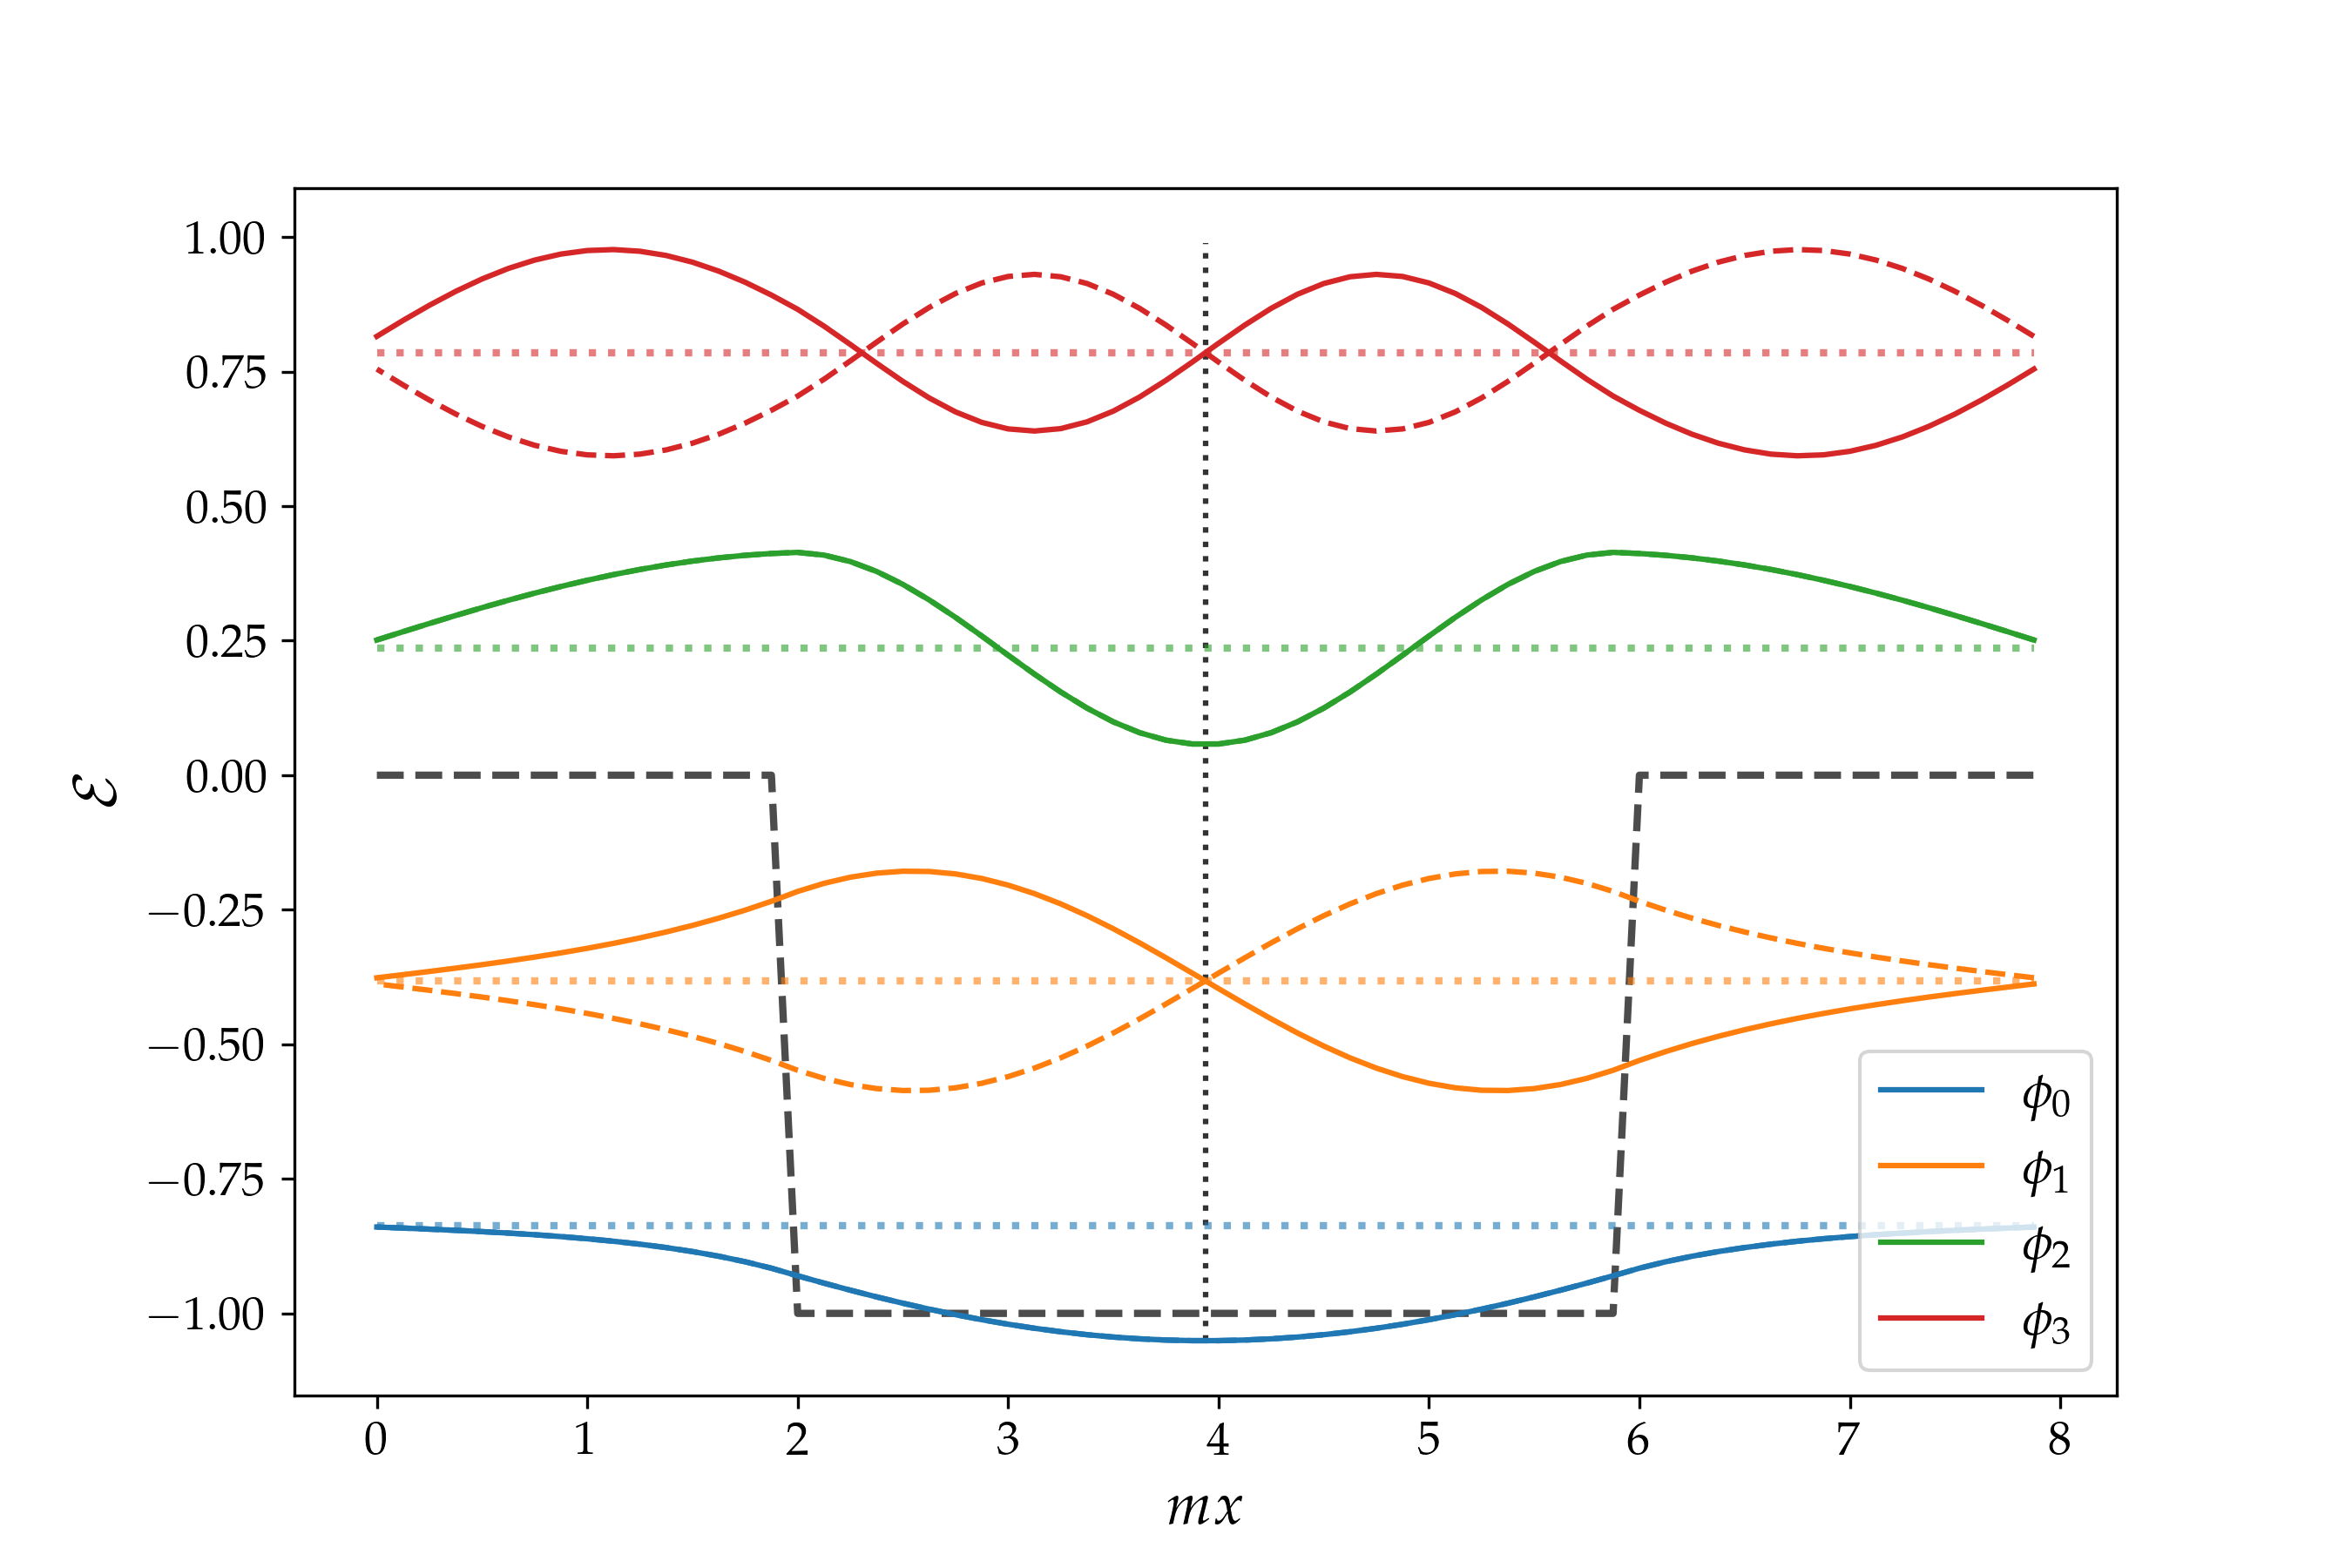
\includegraphics[width=0.7\linewidth]{images/18/finite_well.png}z
    \caption{I primi quattro autostati della buca finita e i relativi autovalori. In linea continua le autofunzioni $\phi_i$, in linea tratteggiata colorata le autofunzioni con parità invertita: $\phi(mx) \to \phi(-mx)$. $\phi_0$ rappresenta il \textit{ground state}. In linea tratteggiata nera il potenziale della buca.}
    \label{fig: fin_well}
\end{figure}

\begin{figure}[H]
    \centering
    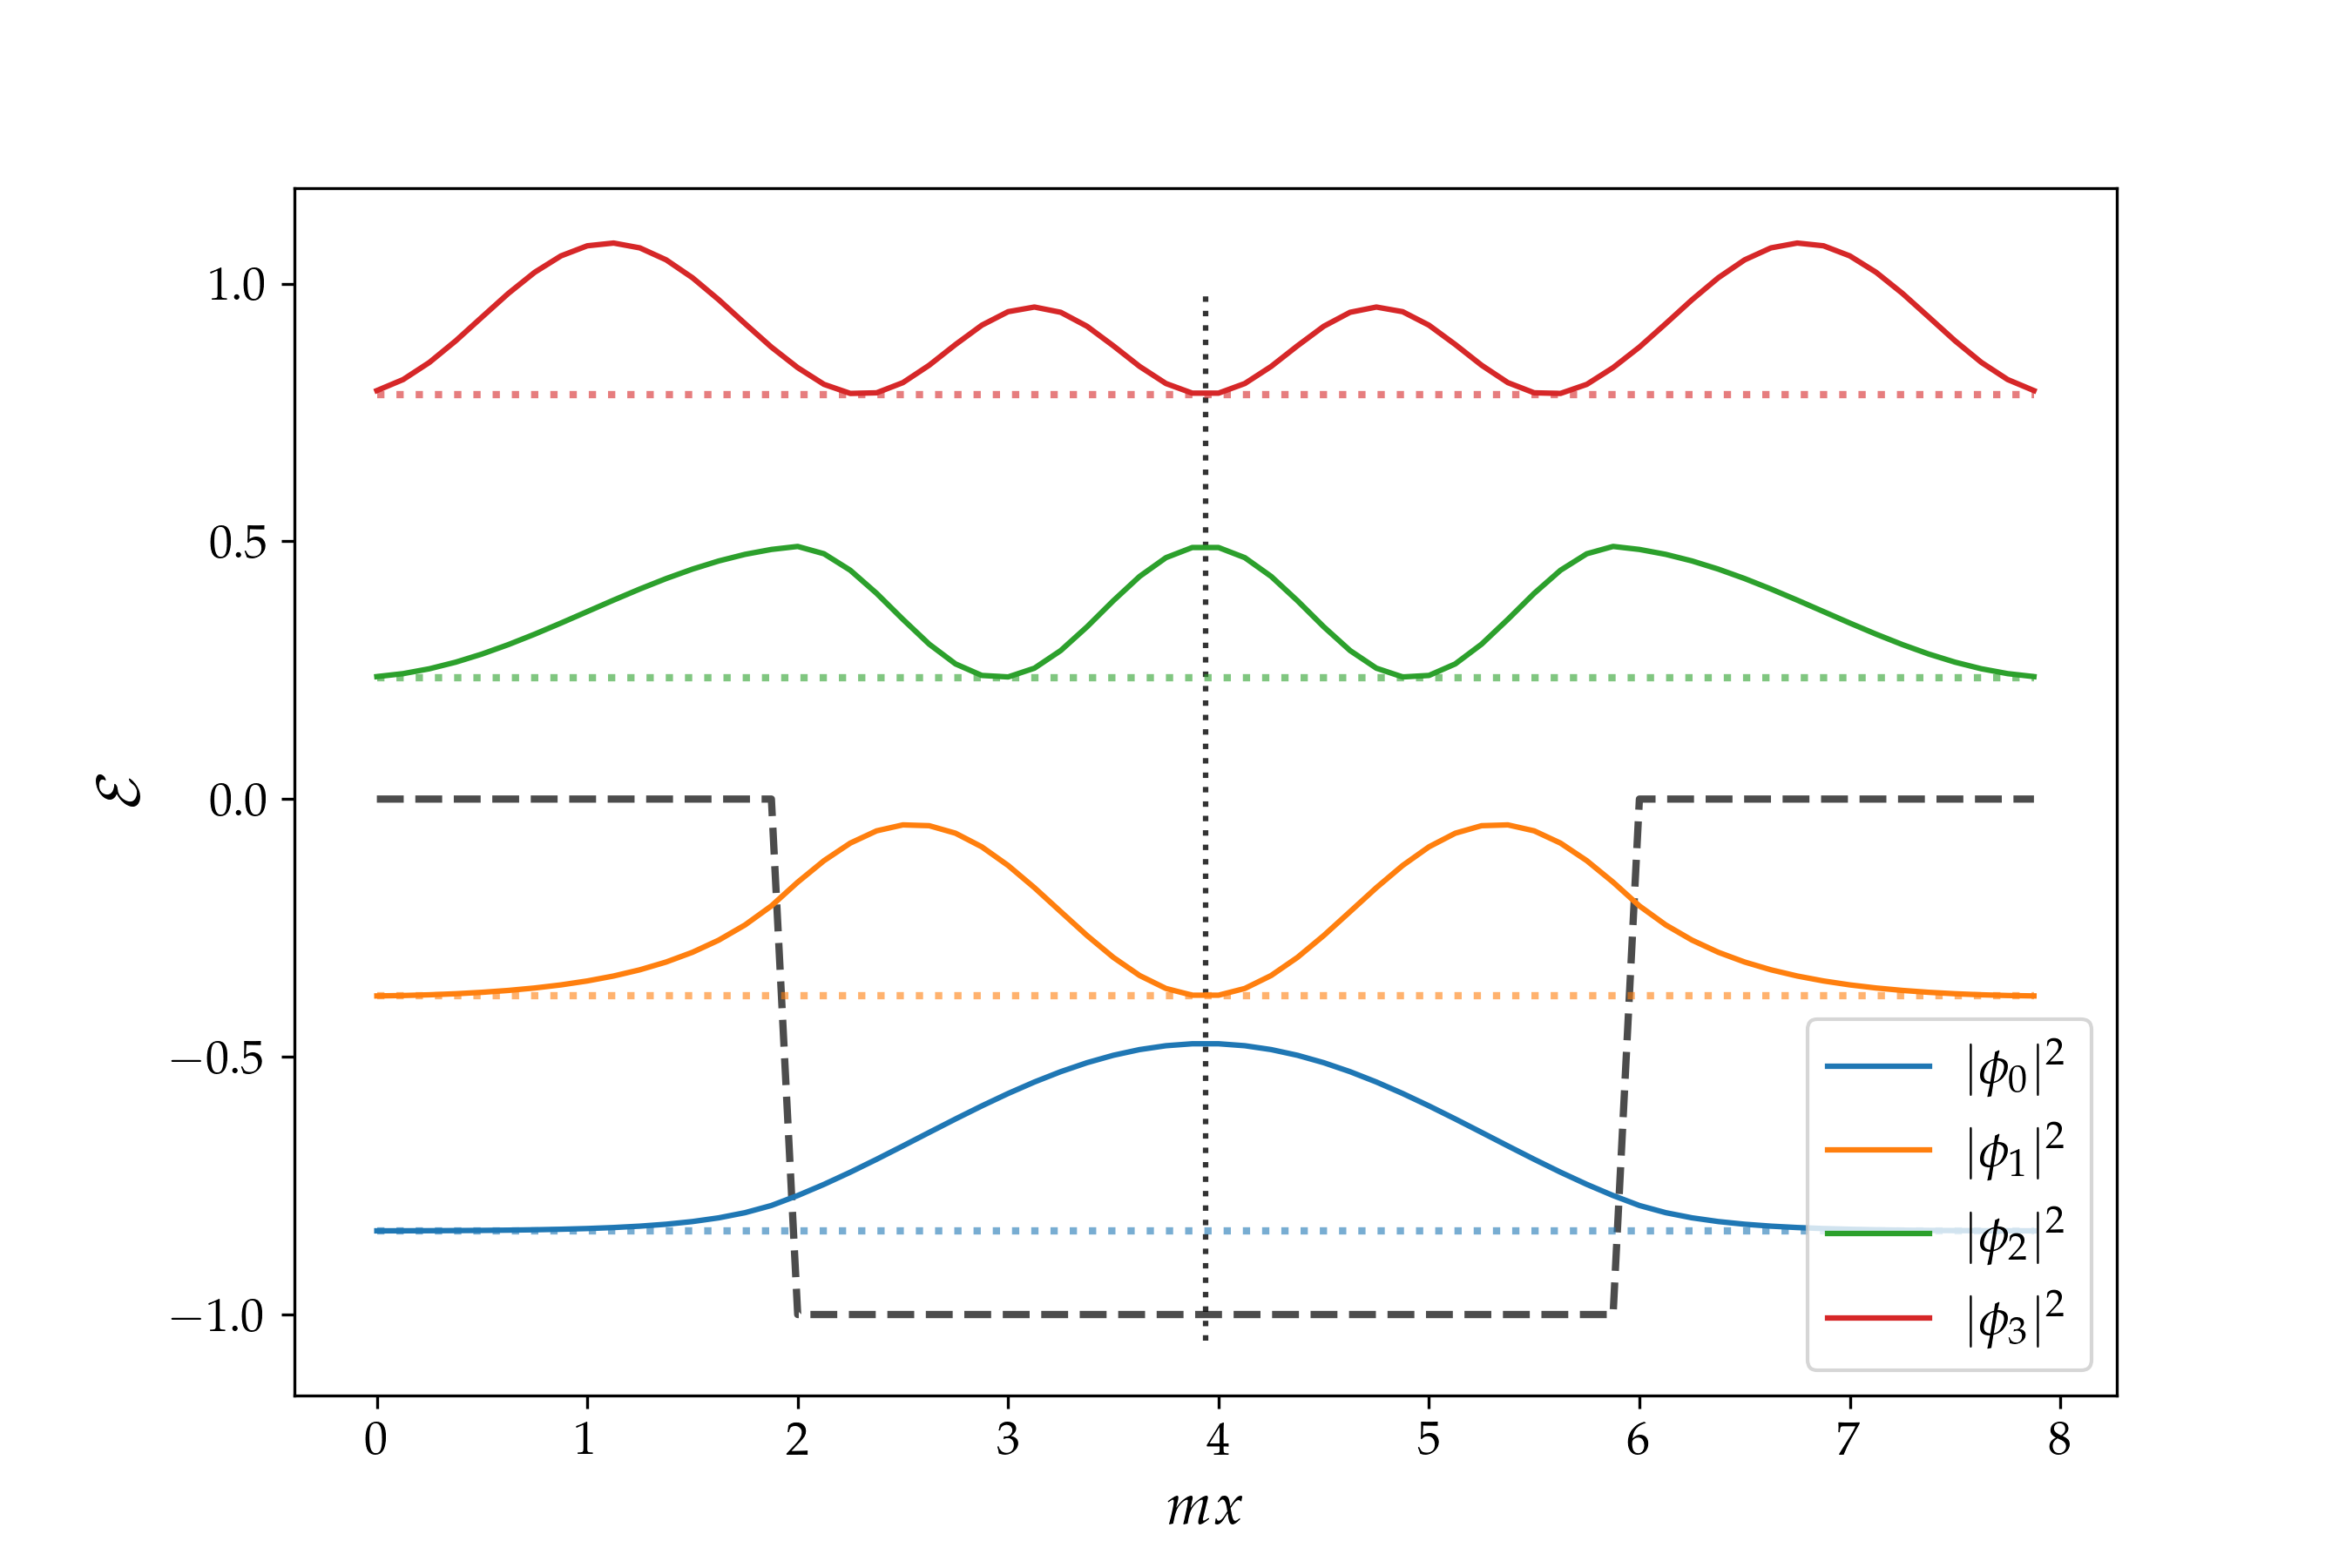
\includegraphics[width=0.7\linewidth]{images/18/finite_well_mod2.png}
    \caption{Modulo quadro dei primi quattro autostati della buca finita.}
    \label{fig: fin_well_mod2}
\end{figure}



\subsubsection{Autostati della barriera finita}
Con $V_0/m = -1$ abbiamo il potenziale di una barriera rettangolare finita. Si osservano due effetti particolari:
\begin{itemize}
    \item Agli autovalori inferiori all'altezza della barriera sono associate autofunzioni che decadono esponenzialmente sotto il potenziale: quello che si osserva è il fenomeno di tunneling quantistico, cioè la probabilità che la particella superi la barriera è non nulla.
    \item Questo sistema evidenzia una simil degenerazione: due livelli energetici sono molto simili\\($\mathcal{E}_1 \approx 0.58, \mathcal{E}_2 \approx 0.59$): in un sistema 1D non è possibile ottenere delle degenerazioni esatte ($\mathcal{E}_i = \mathcal{E}_j$ implicherebbe che le due autofunzioni siano linearmente dipendenti, quindi lo stesso autostato a meno di una fase).
\end{itemize}

\noindent Possiamo immaginare questa configurazione come l'approssimazione di due buche separate da una barriera. Se la barriera è infinita i due sistemi sono isolati e non possono interagire: gli stati fondamentali sono $\psi_L, \psi_R$. Immaginiamo di modificare il sistema e di rendere la barriera finita; le due fdo possono interagire e sovrapporsi. Introducendo l'elemento di matrice $$t=\langle\psi_L|\hat H| \psi_R \rangle = \langle\psi_R|\hat H| \psi_L \rangle$$
che rappresenta il termine di accoppiamento dovuto all'interazione tra $L$ e $R$, possiamo studiare gli autostati/valori di questo nuovo sistema:
\begin{align*}
    H = 
    \begin{pmatrix}
        E_0 & t \\
        t & E_0
    \end{pmatrix}
\end{align*}

dove 
\begin{align*}
    |\psi_L\rangle = \begin{pmatrix}
        1\\
        0
    \end{pmatrix}, \quad    
    |\psi_R\rangle = \begin{pmatrix}
        0\\
        1
    \end{pmatrix}    
\end{align*}

\begin{align*}
    \hat H|\psi_L\rangle &=  E_0 |\psi_L\rangle + t|\psi_R\rangle\\
    \hat H|\psi_R\rangle &=  E_0 |\psi_R\rangle + t|\psi_L\rangle
\end{align*}

diagonalizzando la matrice troviamo gli autovalori, in particolare:
\begin{align*}
    \det(H- EI) & =(E_0- E)^2 - t^2 = 0\\
    \implies \quad & E = E_0 \pm |t|
\end{align*}

\noindent Le autofunzioni associate:
\begin{itemize}

    \item $E = E_0 - |t|$\\
    L'autovettore è 
        \begin{pmatrix}
            1\\
            1
        \end{pmatrix}
    \[
    \boldsymbol v_S = \frac{1}{\sqrt{2}} (|\psi_L\rangle + |\psi_R\rangle)
    \]

    L'autostato sul livello energetico più basso, il \textit{GS}, è quello dato dalla sovrapposizione simmetrica delle due autofunzioni delle buche.

    \item $E = E_0 + |t|$\\
    L'autovettore è 
        \begin{pmatrix}
            1\\
            -1
        \end{pmatrix}
    \[
    \boldsymbol v_A = \frac{1}{\sqrt{2}} (|\psi_L\rangle - |\psi_R\rangle)
    \]
    cioè individuiamo lo stato antisimmetrico come quello più energetico.
\end{itemize}

\noindent Questa separazione sussiste dal momento che abbiamo aggiunto un termine che permette l'interazione tra le due funzioni d'onda, cioè dal momento che abbiamo impostato una barriera finita, cioè che permette tunneling: ci aspettiamo che la separazione dei due stati aumenti all'aumentare dell'interazione tra le due $|\psi_L\rangle, |\psi_R\rangle$, cioè all'abbassarsi della barriera, o al suo assottigliamento. Il caso limite diventa l'eliminazione della stessa, che ci riporta in una configurazione con due stati nettamente separati, cioè quella della buca infinita.\\
D'altra parte vi è il caso della barriera sempre più alta, che fa diminuire l'accoppiamento tra gli stati, avvicinando i livelli energetici. Il caso limite diventa chiaramente quello con cui eravamo partiti; due buche infinite separate. Le due funzioni sono relative ad un potenziale simmetrico, indi per cui le soluzioni sono necessariamente simmetriche (e in questo caso identiche).
\begin{figure}[H]
    \centering
    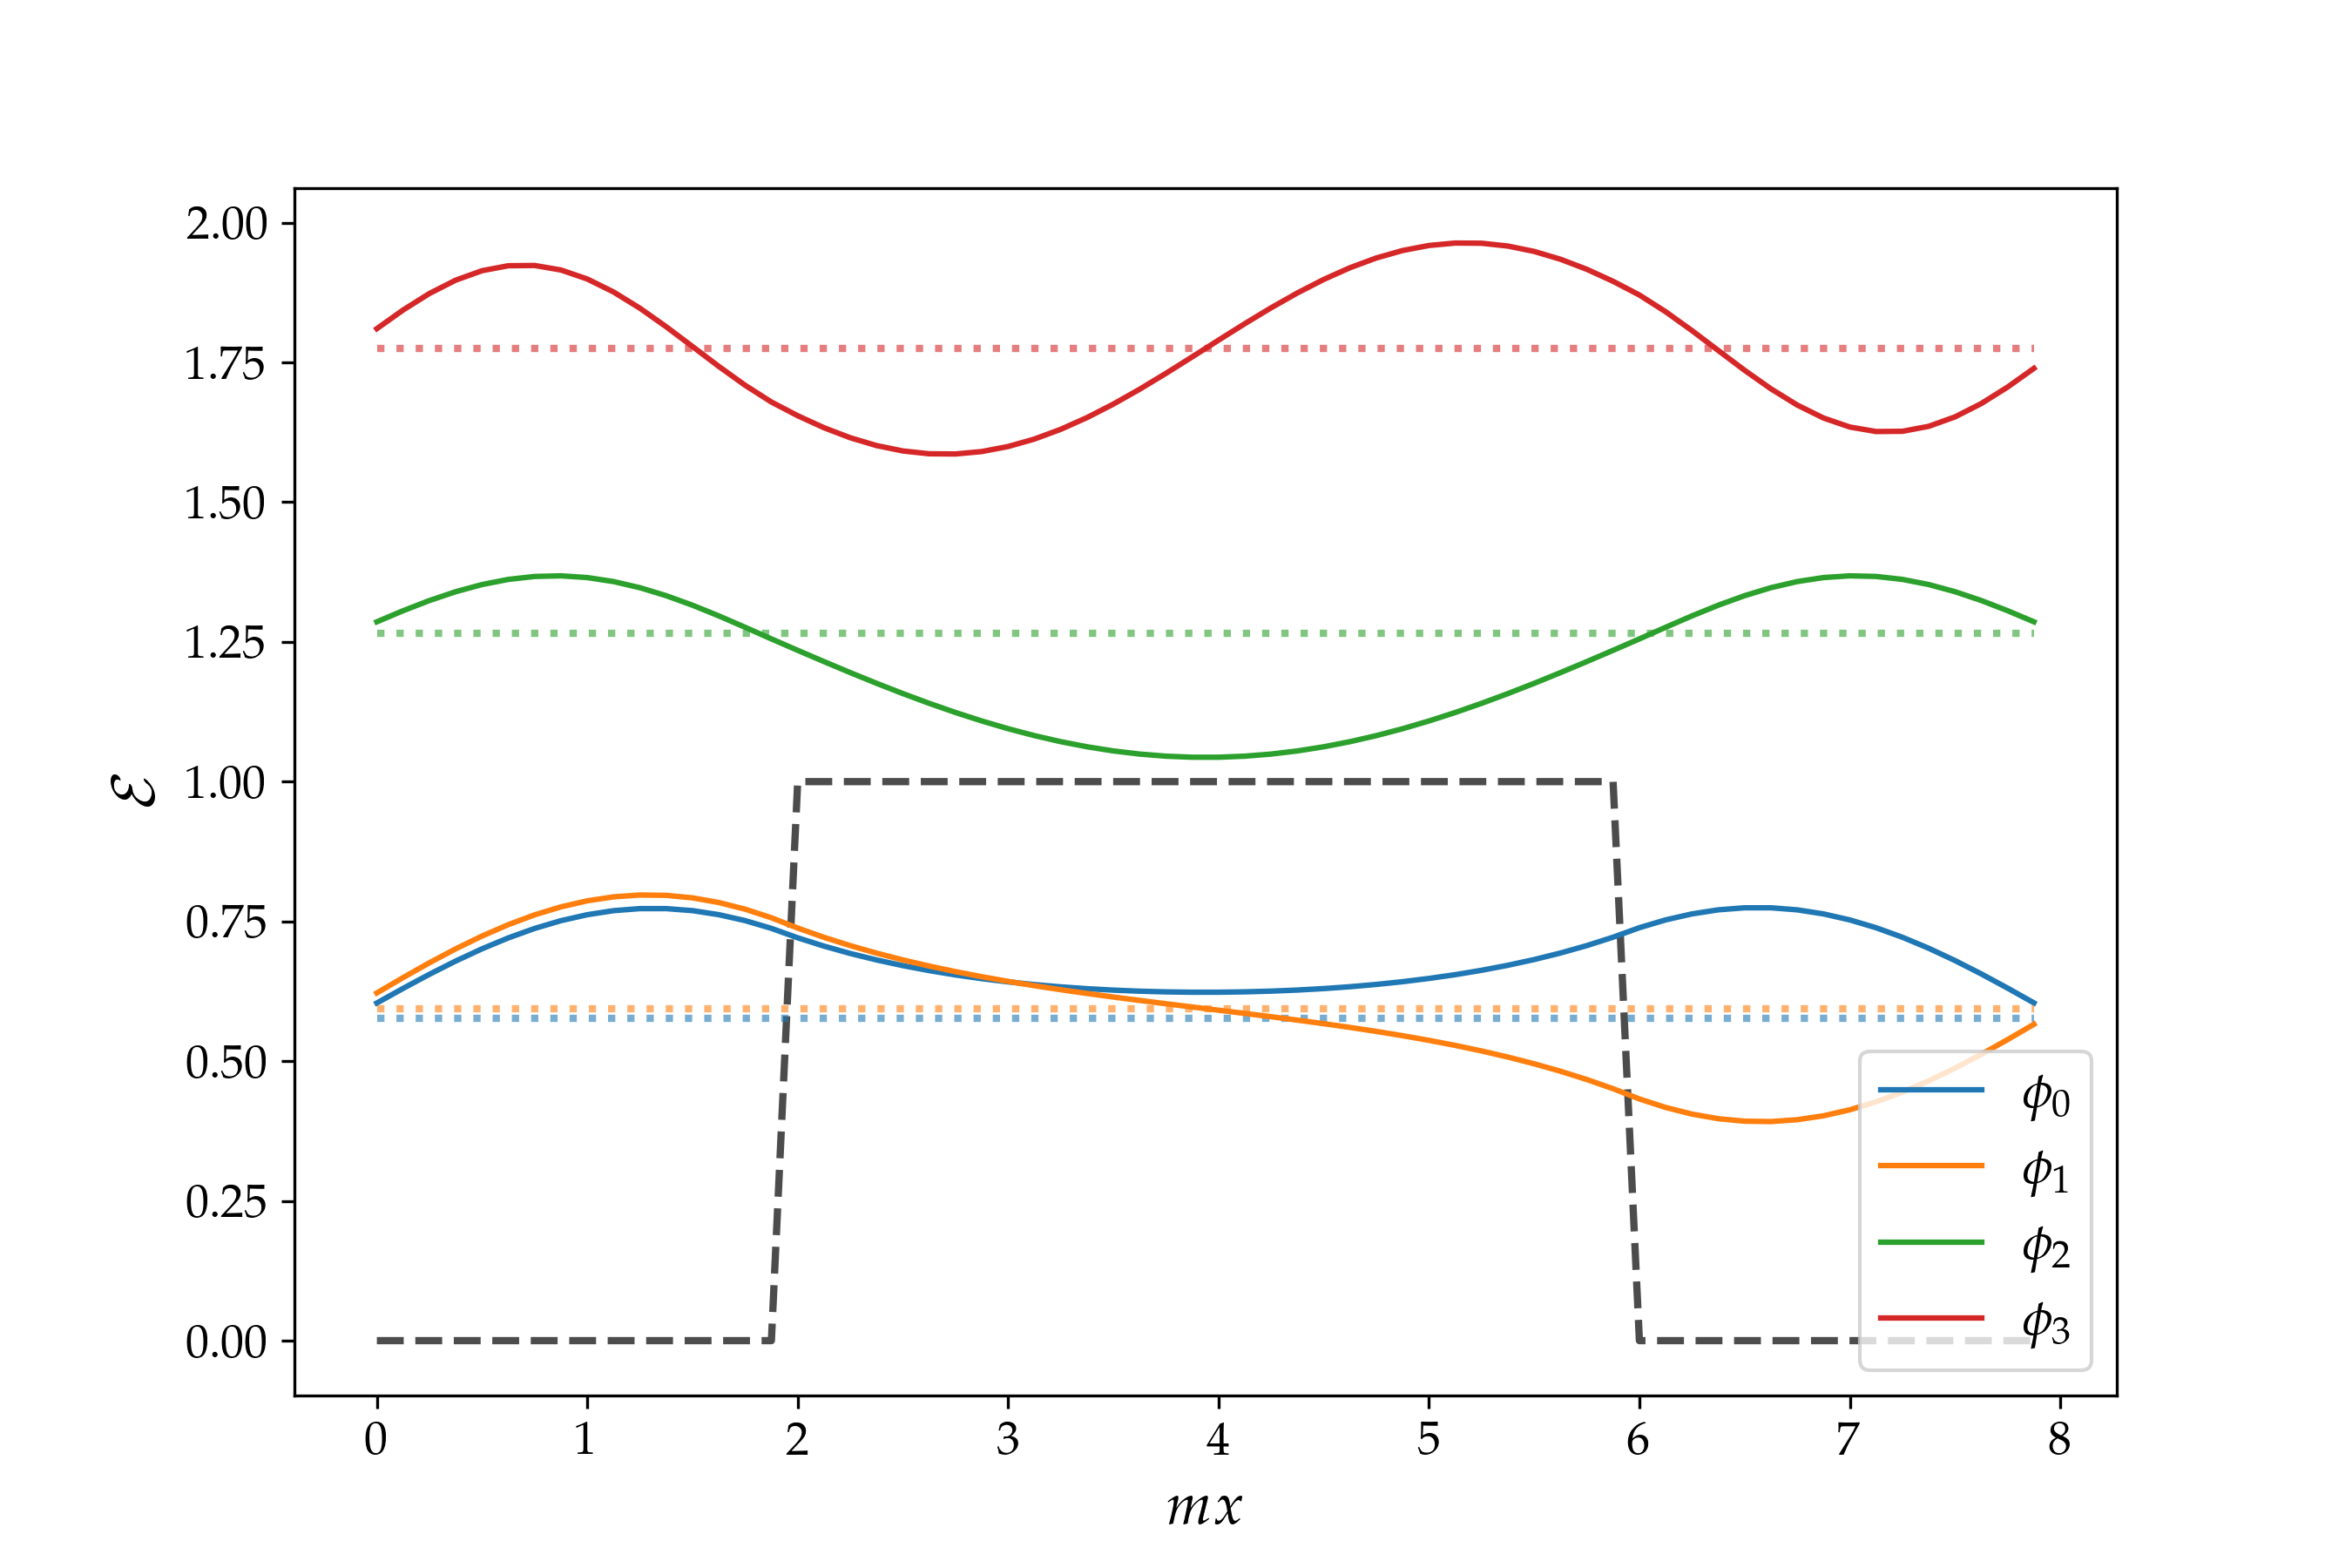
\includegraphics[width=0.7\linewidth]{images/18/finite_wall.png}
    \caption{I primi quattro autostati della barriera finita; si osserva una simil degenerazione per $\phi_0, \phi_1$.}
    \label{fig: fin_wall}
\end{figure}
\begin{figure}[H]
    \centering
    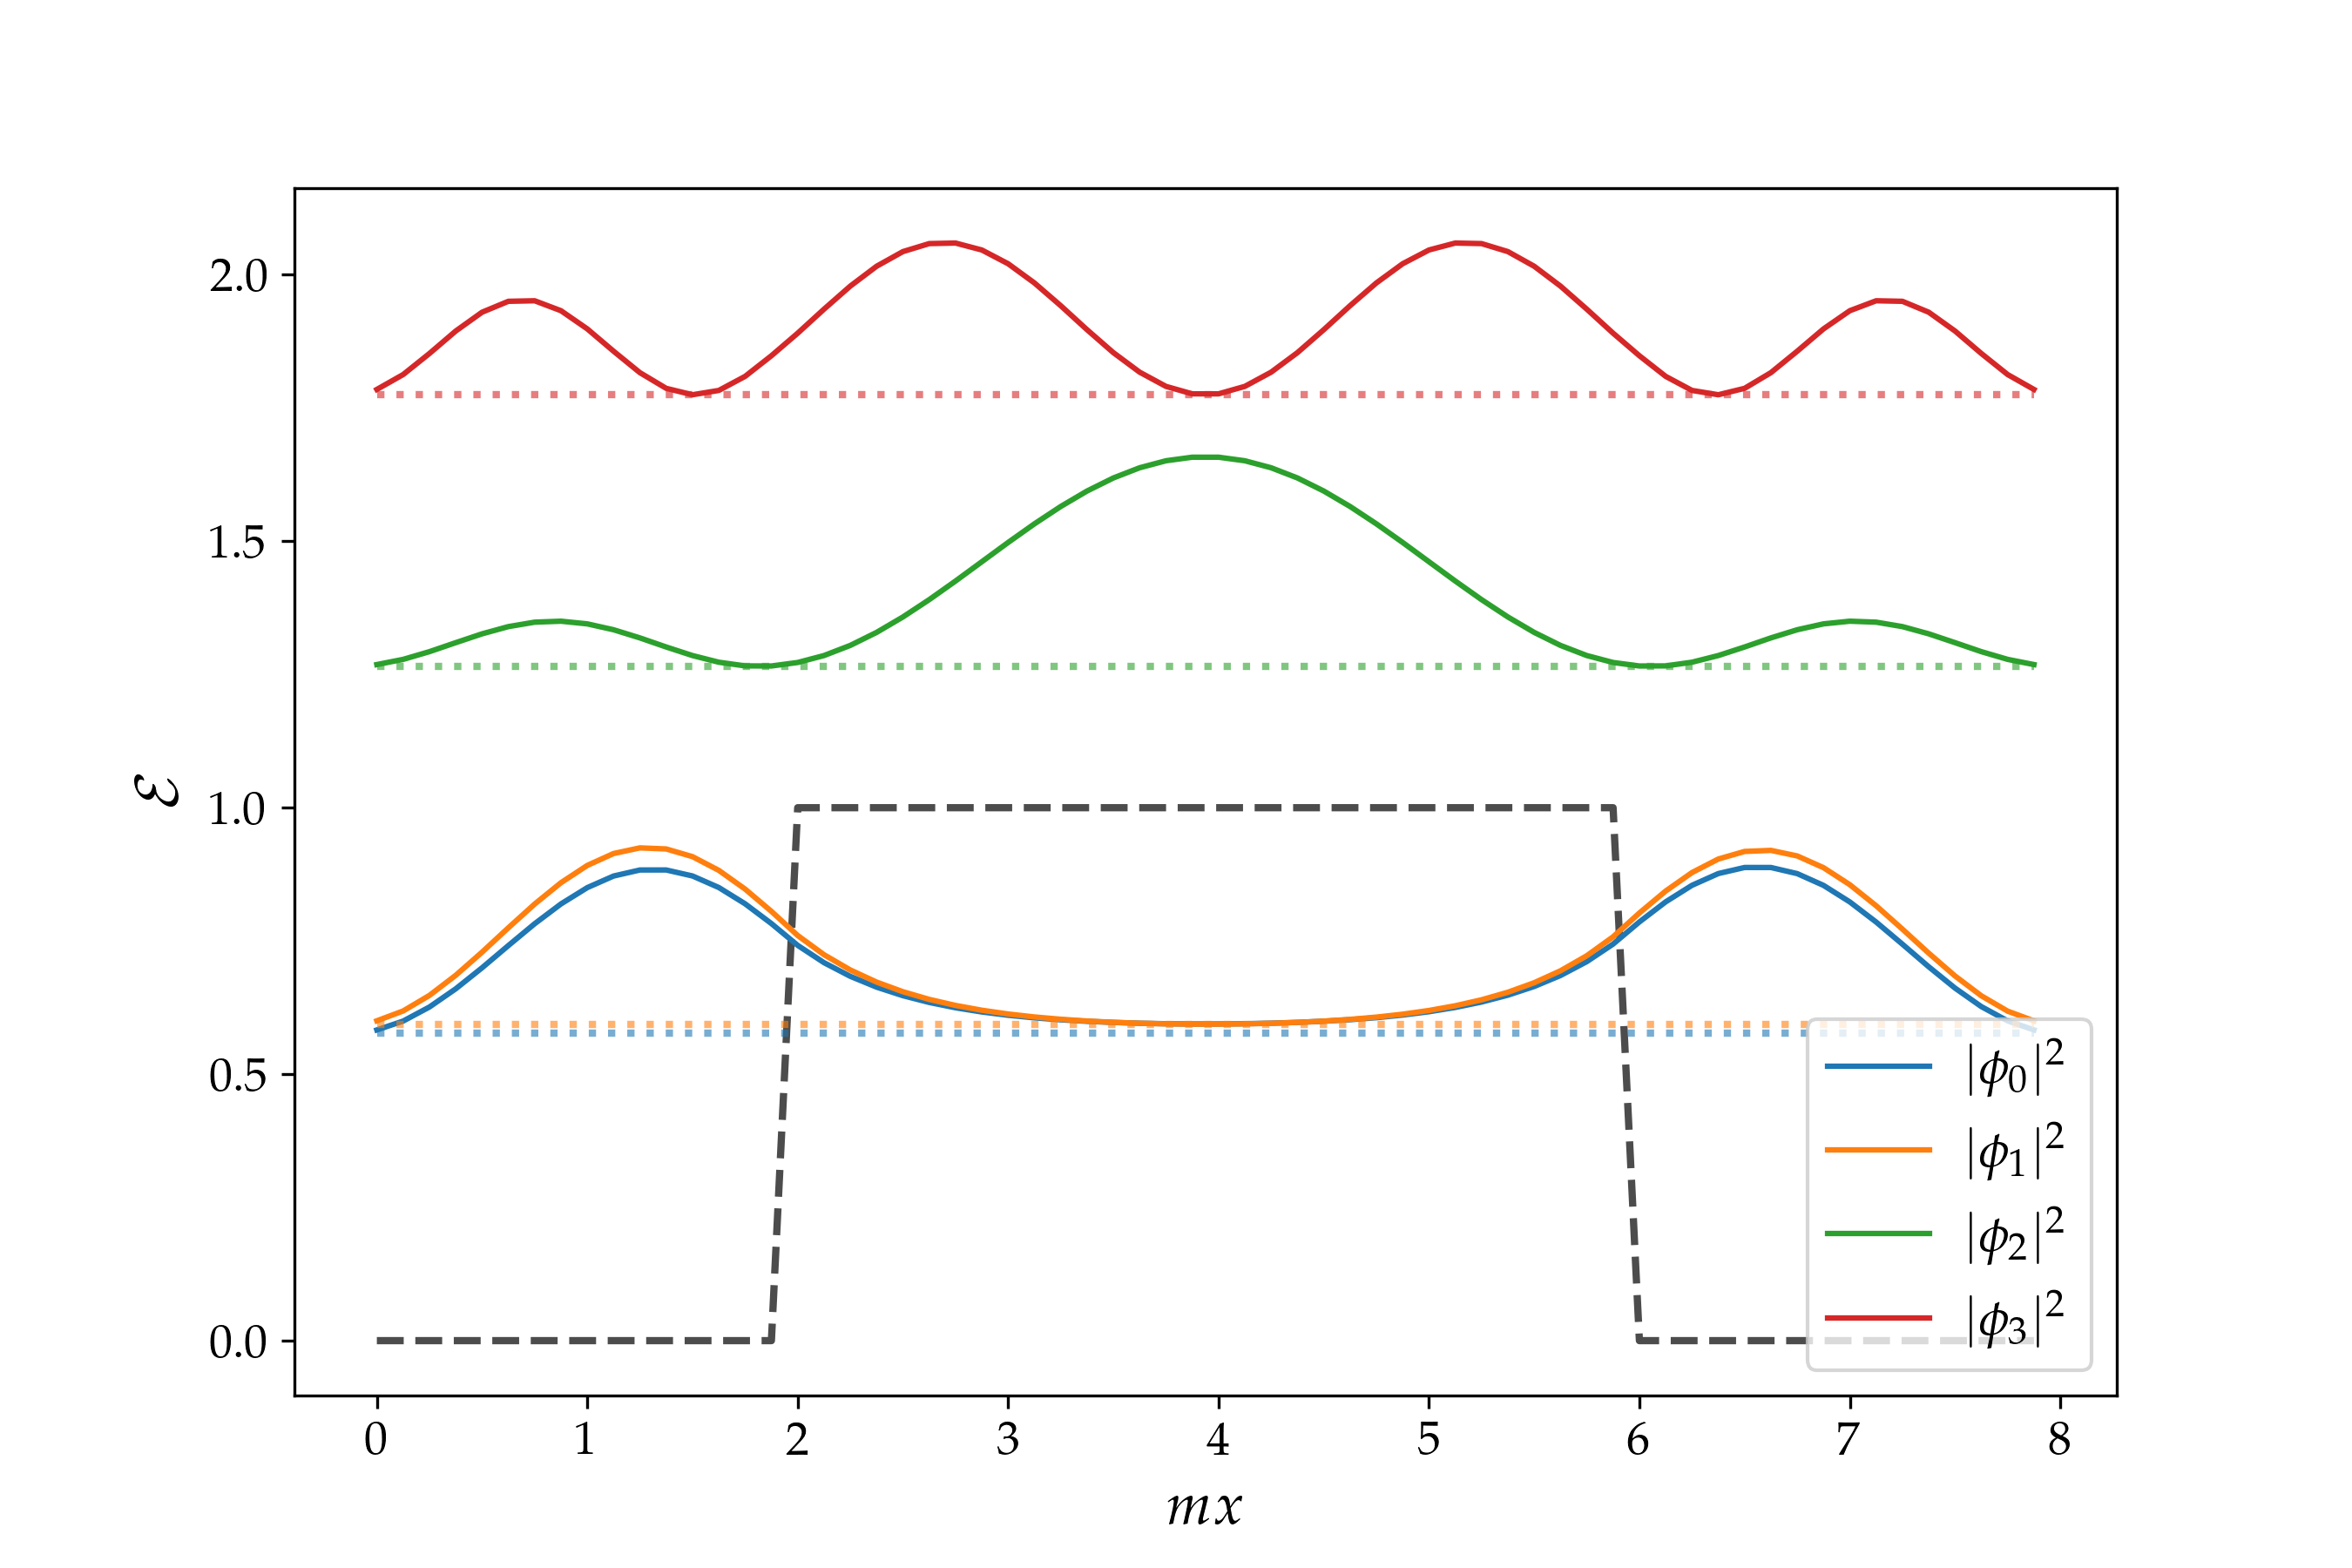
\includegraphics[width=0.7\linewidth]{images/18/finite_wall_mod2.png}
    \caption{Modulo quadro dei primi quattro autostati della barriera finita.}
    \label{fig: fin_wall_mod2}
\end{figure}




\subsubsection{Stati fondamentali al variare di $V_0/m$}
Tornando al caso della buca finita, studiamo cosa accade all'aumentare della profondita di questa: come si trasforma la funzione d'onda?\\
Quello che stiamo studiando è effettivamente l'approssimazione crescente a una buca infinita, la cui soluzione esatta è nota: gli autostati sono le funzioni
$$\psi_n(x) = \begin{cases} \sqrt{\frac{2}{b - a}} \sin\left(\frac{n\pi(x - a)}{b - a}\right) & a < x < b \\ 0 & \text{altrove} \end{cases}$$
\[
n=1,2,3, \dots
\]

di cui il \textit{GS}:
\[
\psi_{GS} = \sqrt{\frac{2}{b - a}} \sin\left(\frac{\pi(x - a)}{b - a}\right)
\]
dove il potenziale della buca infinita tra due estremi $a, b$ è definito come:
\[
V(x) = \begin{cases}
    0 & a<x<b\\
    +\infty & \text{altrove}
\end{cases}
\]

\noindent Concludiamo quindi che in Fig. \ref{fig: well_var} si osserva questa tendenza: si noti come diminuisca la profondità di perforazione della barriera nella regione proibita che la funzione d'onda riesce ad avere per via della decrescenza esponenziale sempre più rapida (che nel limite di barriera infinita fissa dei nodi nei punti $a, b$). 


\begin{figure}[H]
    \centering
    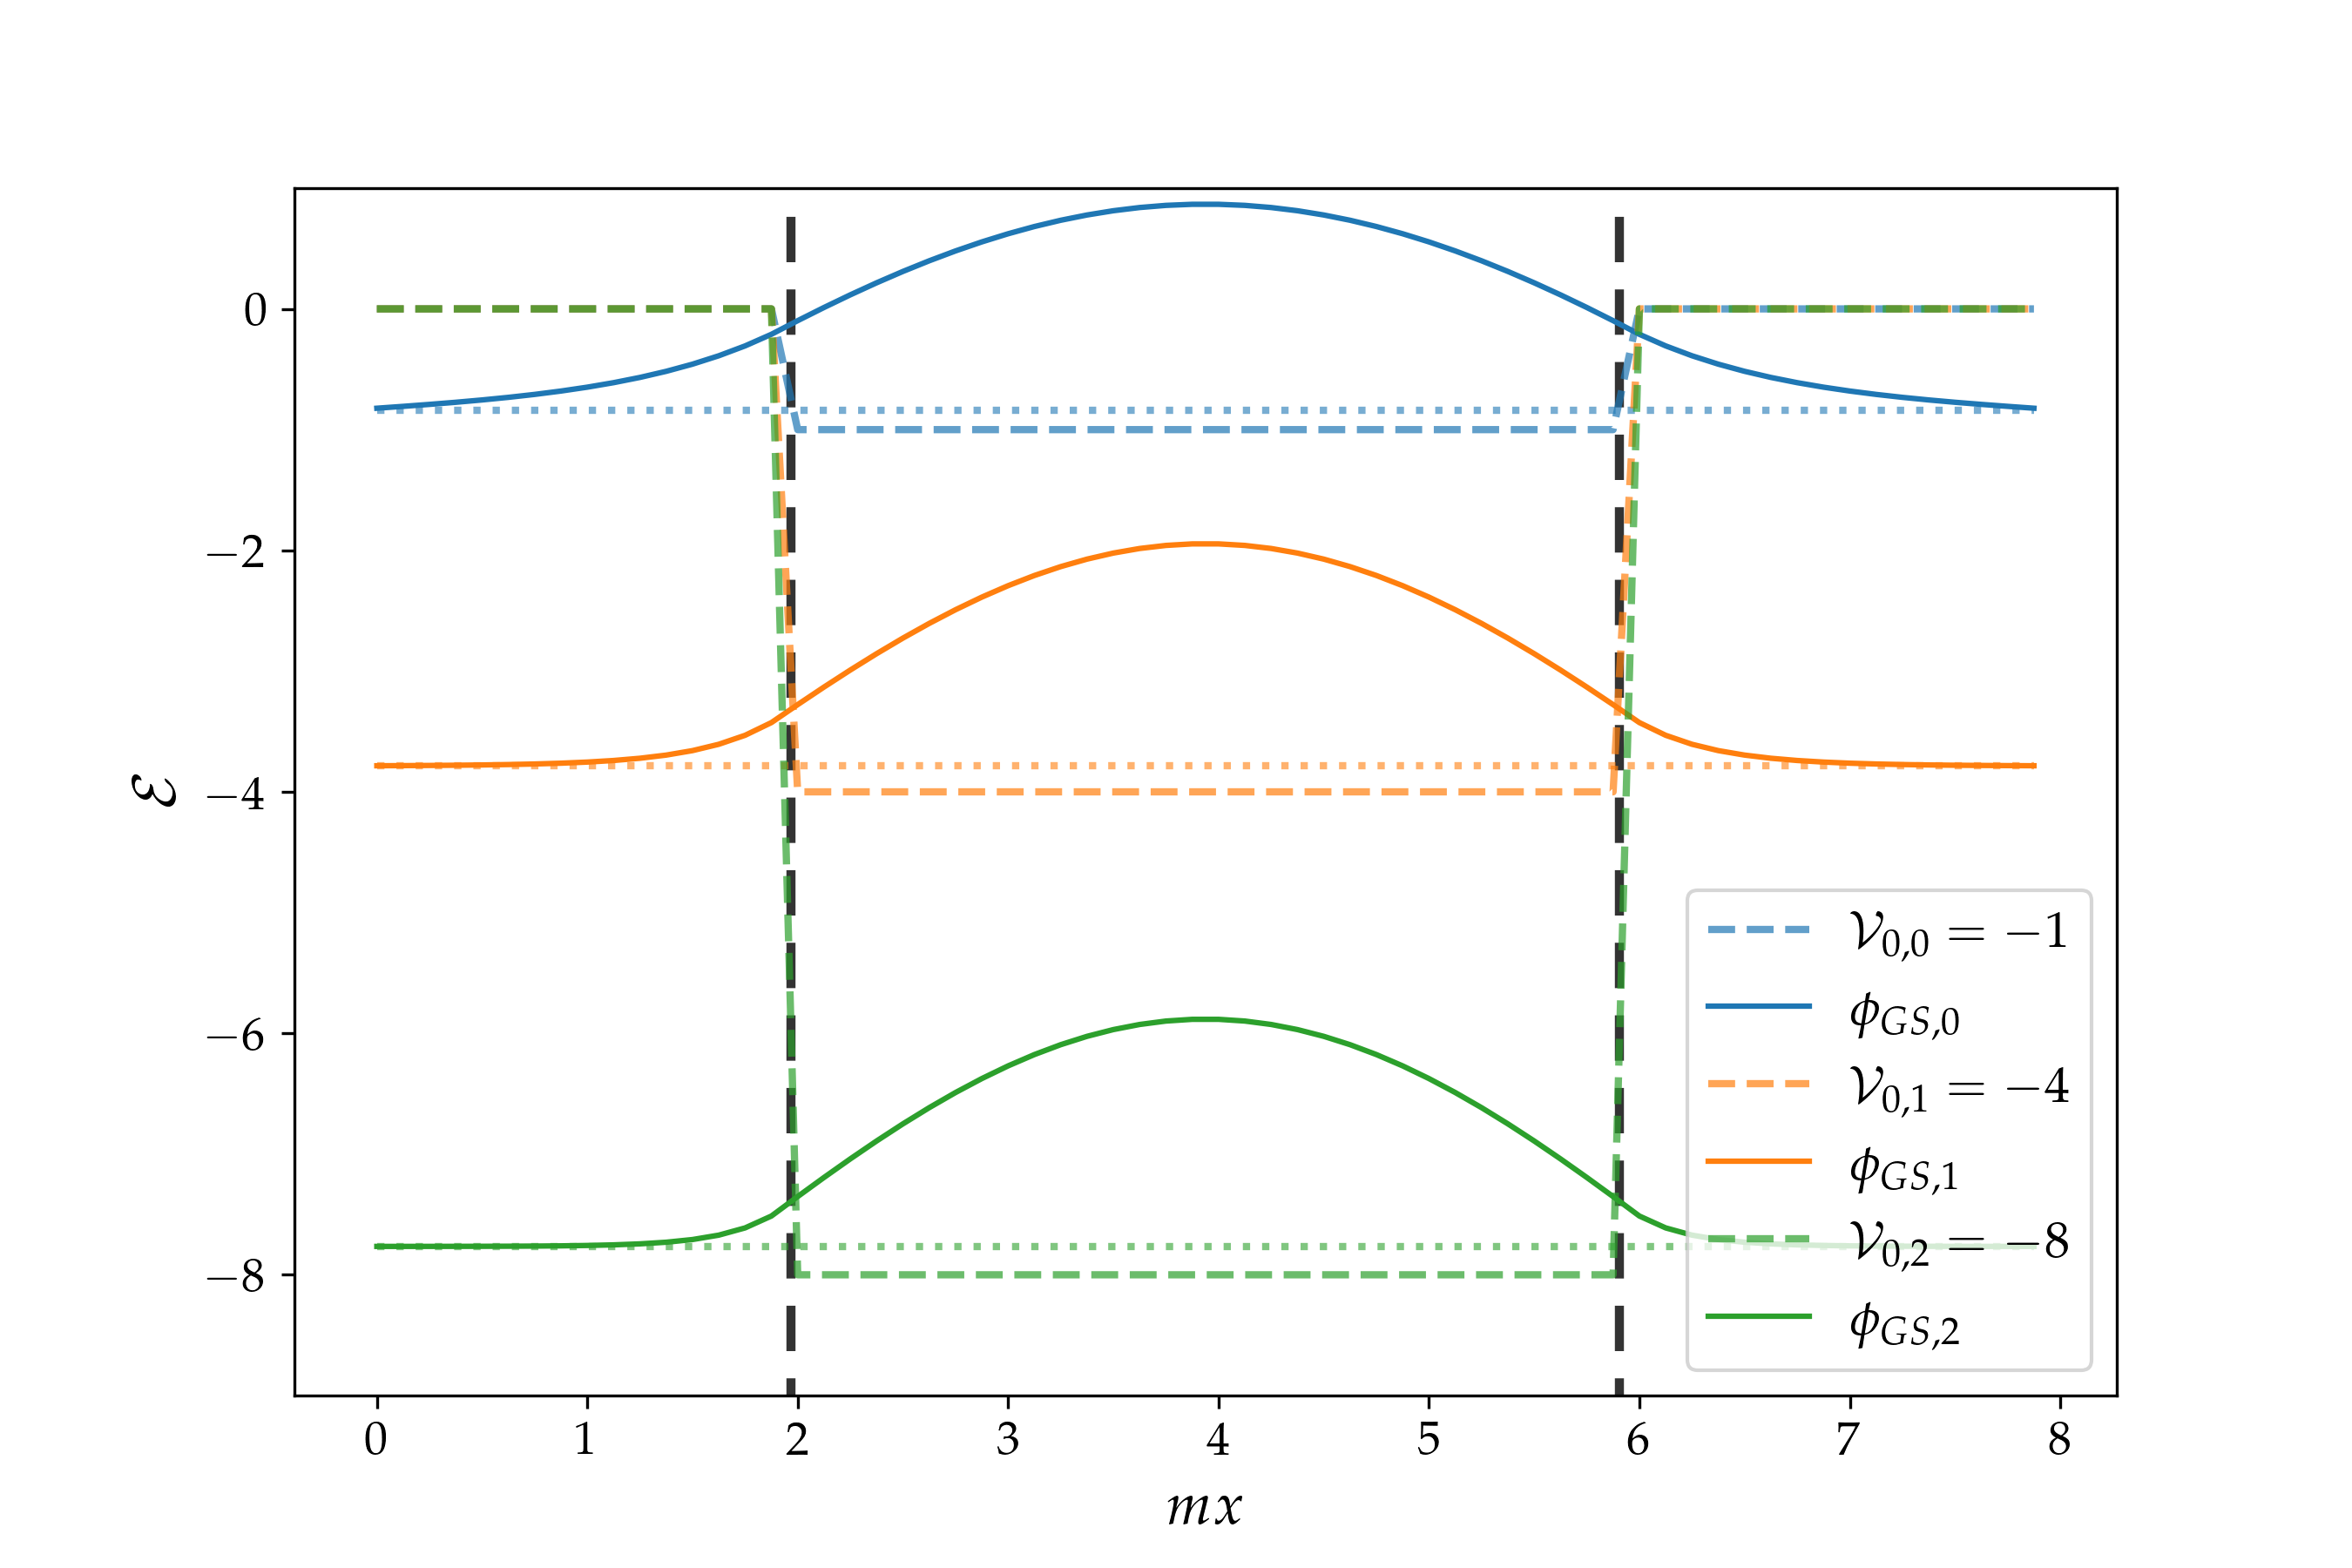
\includegraphics[width=0.8\linewidth]{images/18/diff_well.png}
    \caption{\textit{Ground states} della buca finita, con diversi valori di $V_0/m \in \{1, 4, 8\}$.}
    \label{fig: well_var}
\end{figure}

\subsubsection{Scaling degli autovalori in funzione di $N$}
Fissando un potenziale di riferimento (nel nostro caso la buca finita) e studiando l'andamento degli $i$-esimi autovalori in funzione della discretizzazione spaziale $N$, si osserva che la velocità di convergenza verso il valore esatto non è uniforme per tutti gli stati.
Per visualizzare meglio il fenomeno, in Fig. \ref{fig: scaling_eval N} abbiamo rappresentato gli autovalori normalizzati rispetto alla loro migliore approssimazione (quella relativa alla massima risoluzione, $\lambda_{64}$), facendo sì che tutti convergano asintoticamente a 1. 
Dal grafico emergono i seguenti comportamenti
\begin{itemize}
    \item Autovalori minori: l'approssimazione risulta sufficientemente accurata anche a basse risoluzioni (valori di $N$ piccoli).
    \item Autovalori maggiori (stati ad alta energia): un $N$ piccolo restituisce un'approssimazione scadente. Poiché $N$ definisce la densità del campionamento sul quale valutiamo la funzione e la sua derivata seconda (approssimata tramite differenze finite), le autofunzioni più energetiche richiedono un reticolo molto più fitto per essere modellate in modo corretto.
    \item Stato fondamentale ($\lambda_1$): costituisce un caso limite, in quanto si osserva che l'errore sul calcolo di questo autovalore si mantiene pressoché costante $\forall N$.
\end{itemize}


\begin{figure}[H]
    \centering
    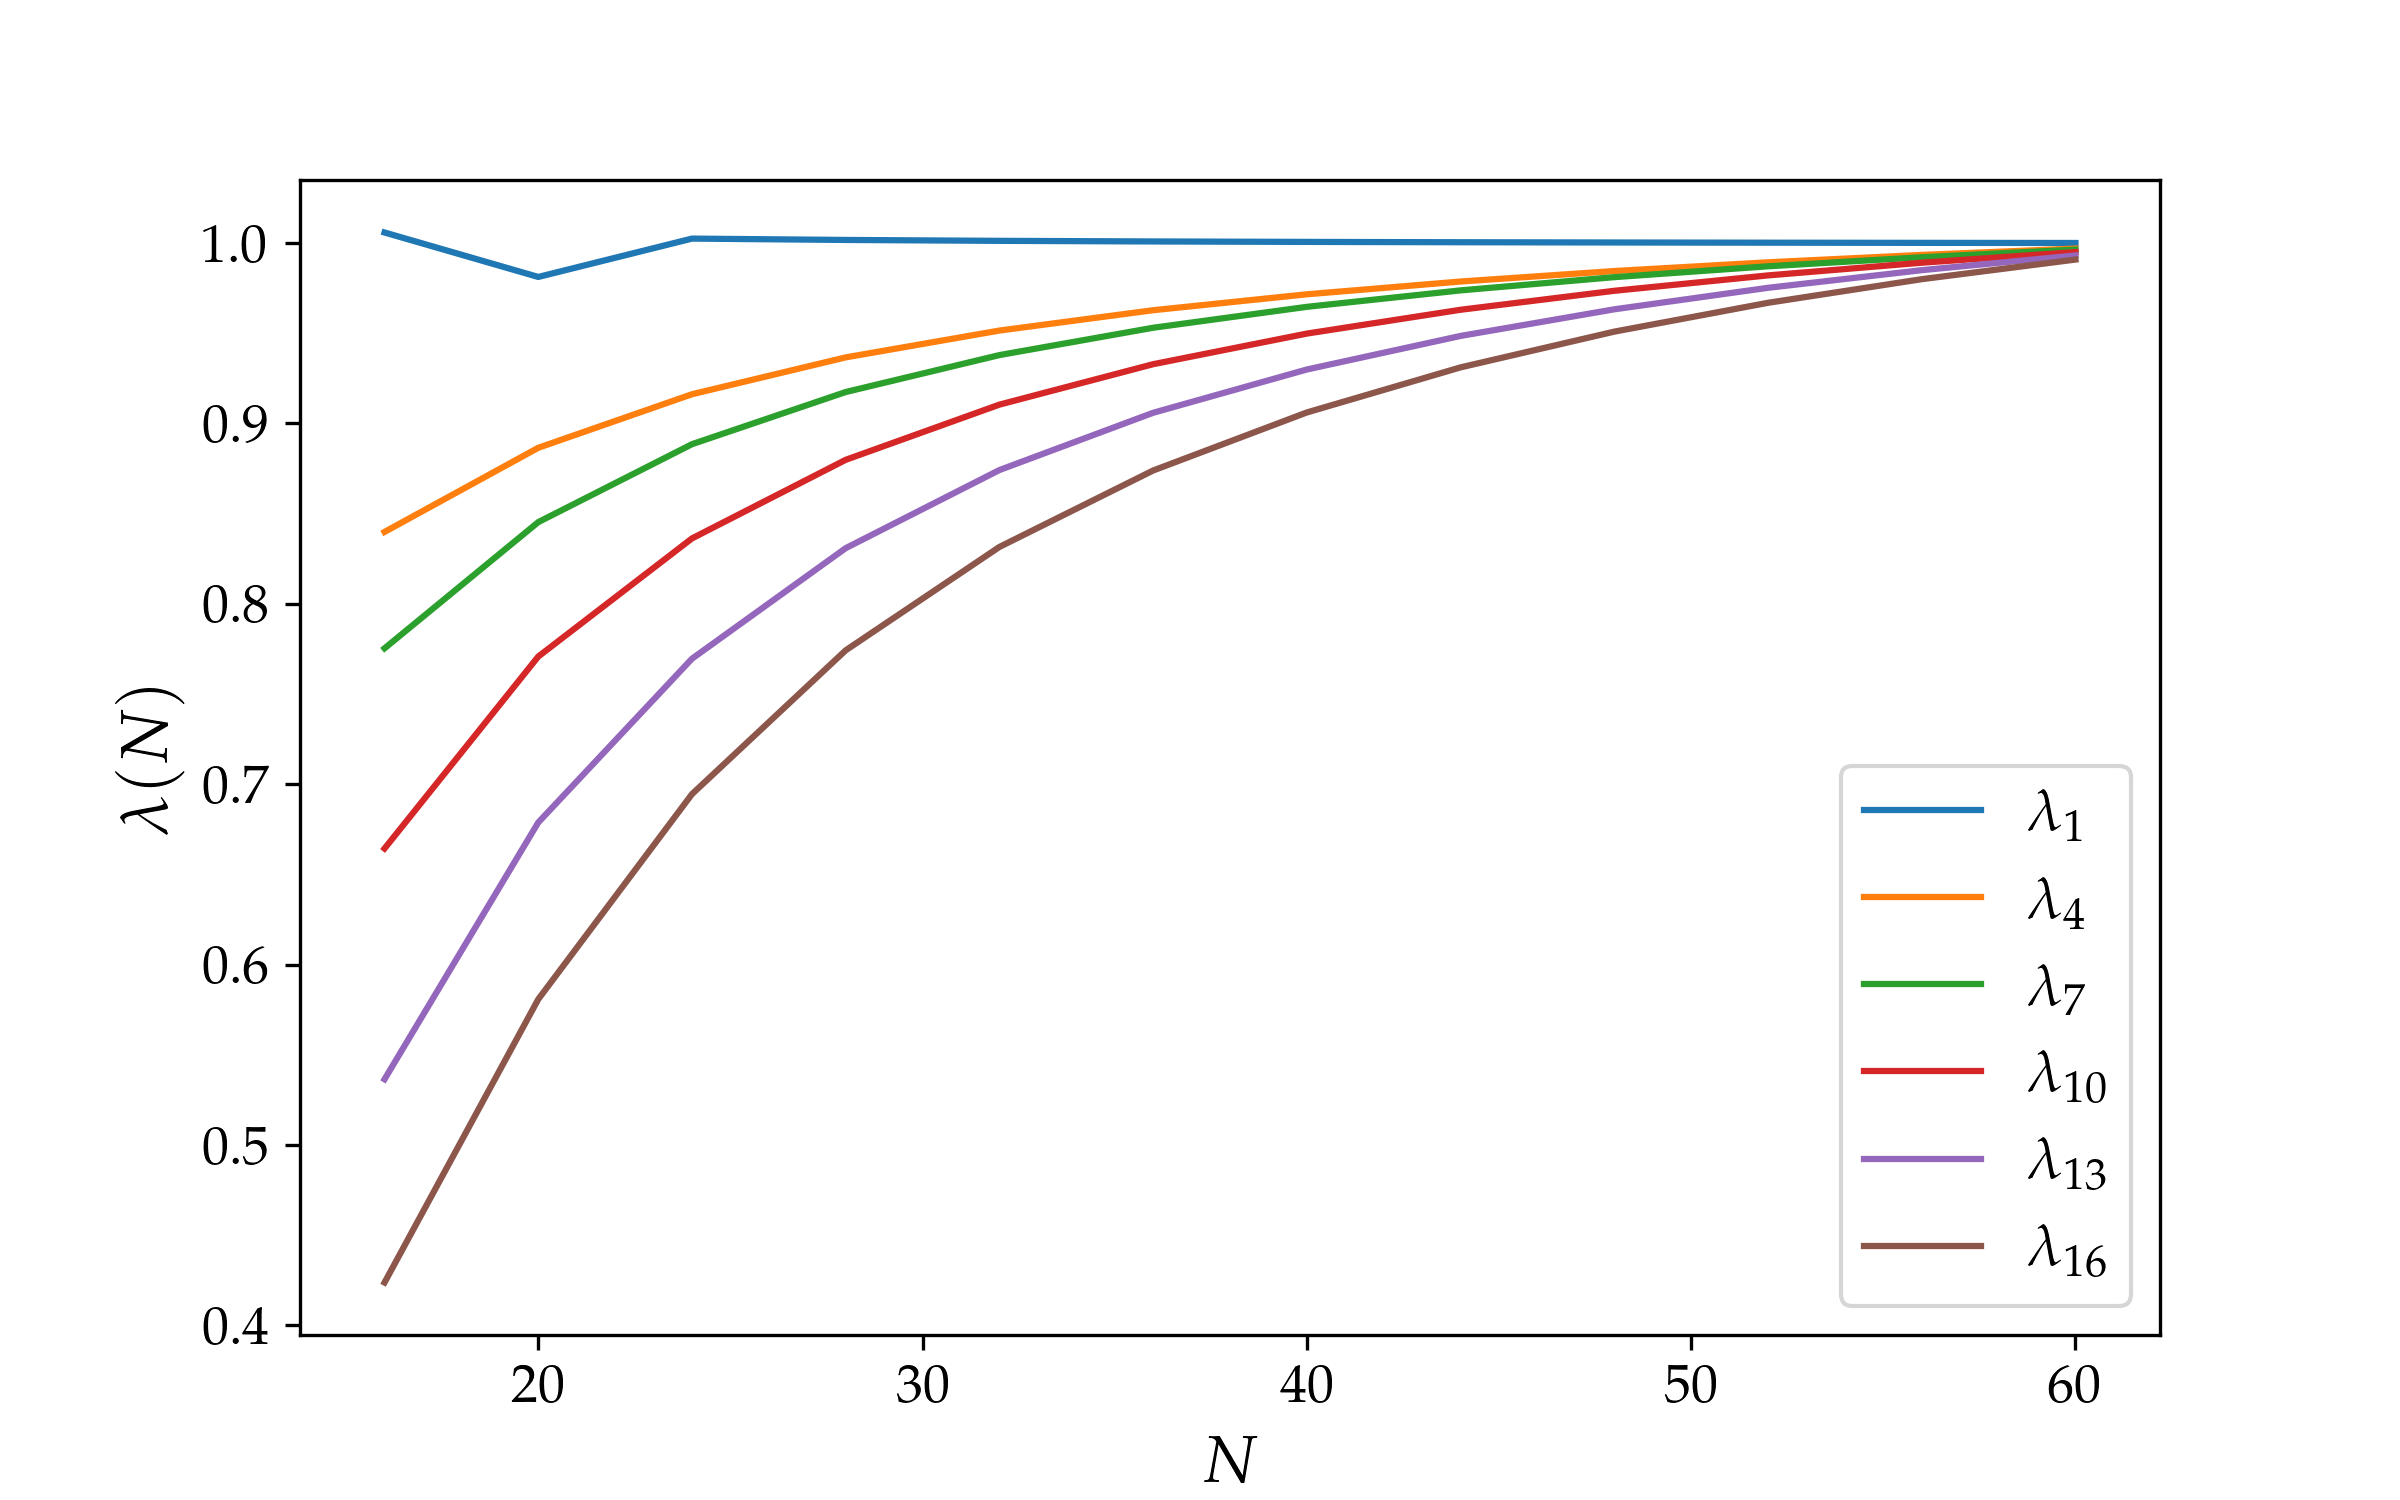
\includegraphics[width=0.8\linewidth]{images/18/rate_N.png}
    \caption{Rate di convergenza degli autovalori i-esimi in funzione di $N$.}
    \label{fig: scaling_eval N}
\end{figure}

\subsubsection{Soluzioni per diversi potenziali statici}
Infine desideriamo dare una breve descrizione del risultato che si può ottenere al variare della forma del potenziale. Delle considerazioni di interesse fisico possono essere fatte sulle soluzioni relative a questi potenziali, ma in questo caso lasciamo la semplice definizione dei potenziali, i loro parametri per i plot e la figura esplicativa Fig. \ref{fig: Diff Pot}.

\medskip\noindent
La buca finita è già stata discussa ampiamente nelle precedenti sezioni, la riproponiamo per il confronto con i casi adiacenti.

\medskip\noindent
La \textbf{buca doppia} è definita da:
$$V(x) = a x^4 - b x^2$$
nel mio codice in particolare applico una traslazione e una dilatazione:
$$x = \frac{u - \frac{N}{2}}{8},\ a=1/2 ,\ b=2$$

\medskip\noindent
Il \textbf{potenziale triangolare} è proprio di un campo di forza costante (per esempio il campo elettrico all'interno di un condensatore):
$$V(x) = \begin{cases} +\infty & \text{se } x < a \\ m \left(x - a\right) & \text{se } x \ge a
\end{cases}$$

i parametri sono stati impostati a:
\[
a=\frac{N}{4}, m = 0.3
\]

\medskip\noindent
Il \textbf{potenziale alfa} è invece quello relativo alle interazioni nucleari:
\begin{enumerate}
    \item Un pozzo attraente, derivato dalla forza nucleare forte a corto raggio, confina una particella poco energetica all'interno del nucleo
    \item Un potenziale coulombiano definisce una barriera respingente, ma che uno stato sufficientemente energetico può superare per tunneling quantistico. Questo fenomeno, descritto anche da Gamow, permette di descrivere per esempio l'emissione di particelle alfa energetiche.
\end{enumerate}

$$V(x) = \begin{cases} -V_0 & \text{se } x < R \\ \frac{k}{x - x_0} & \text{se } x \ge R \end{cases}$$

nel codice queste le impostazioni:
\[
R = \frac{N}{4}, k = 2, x_0=15
\]


\begin{figure}[H]
    \centering
    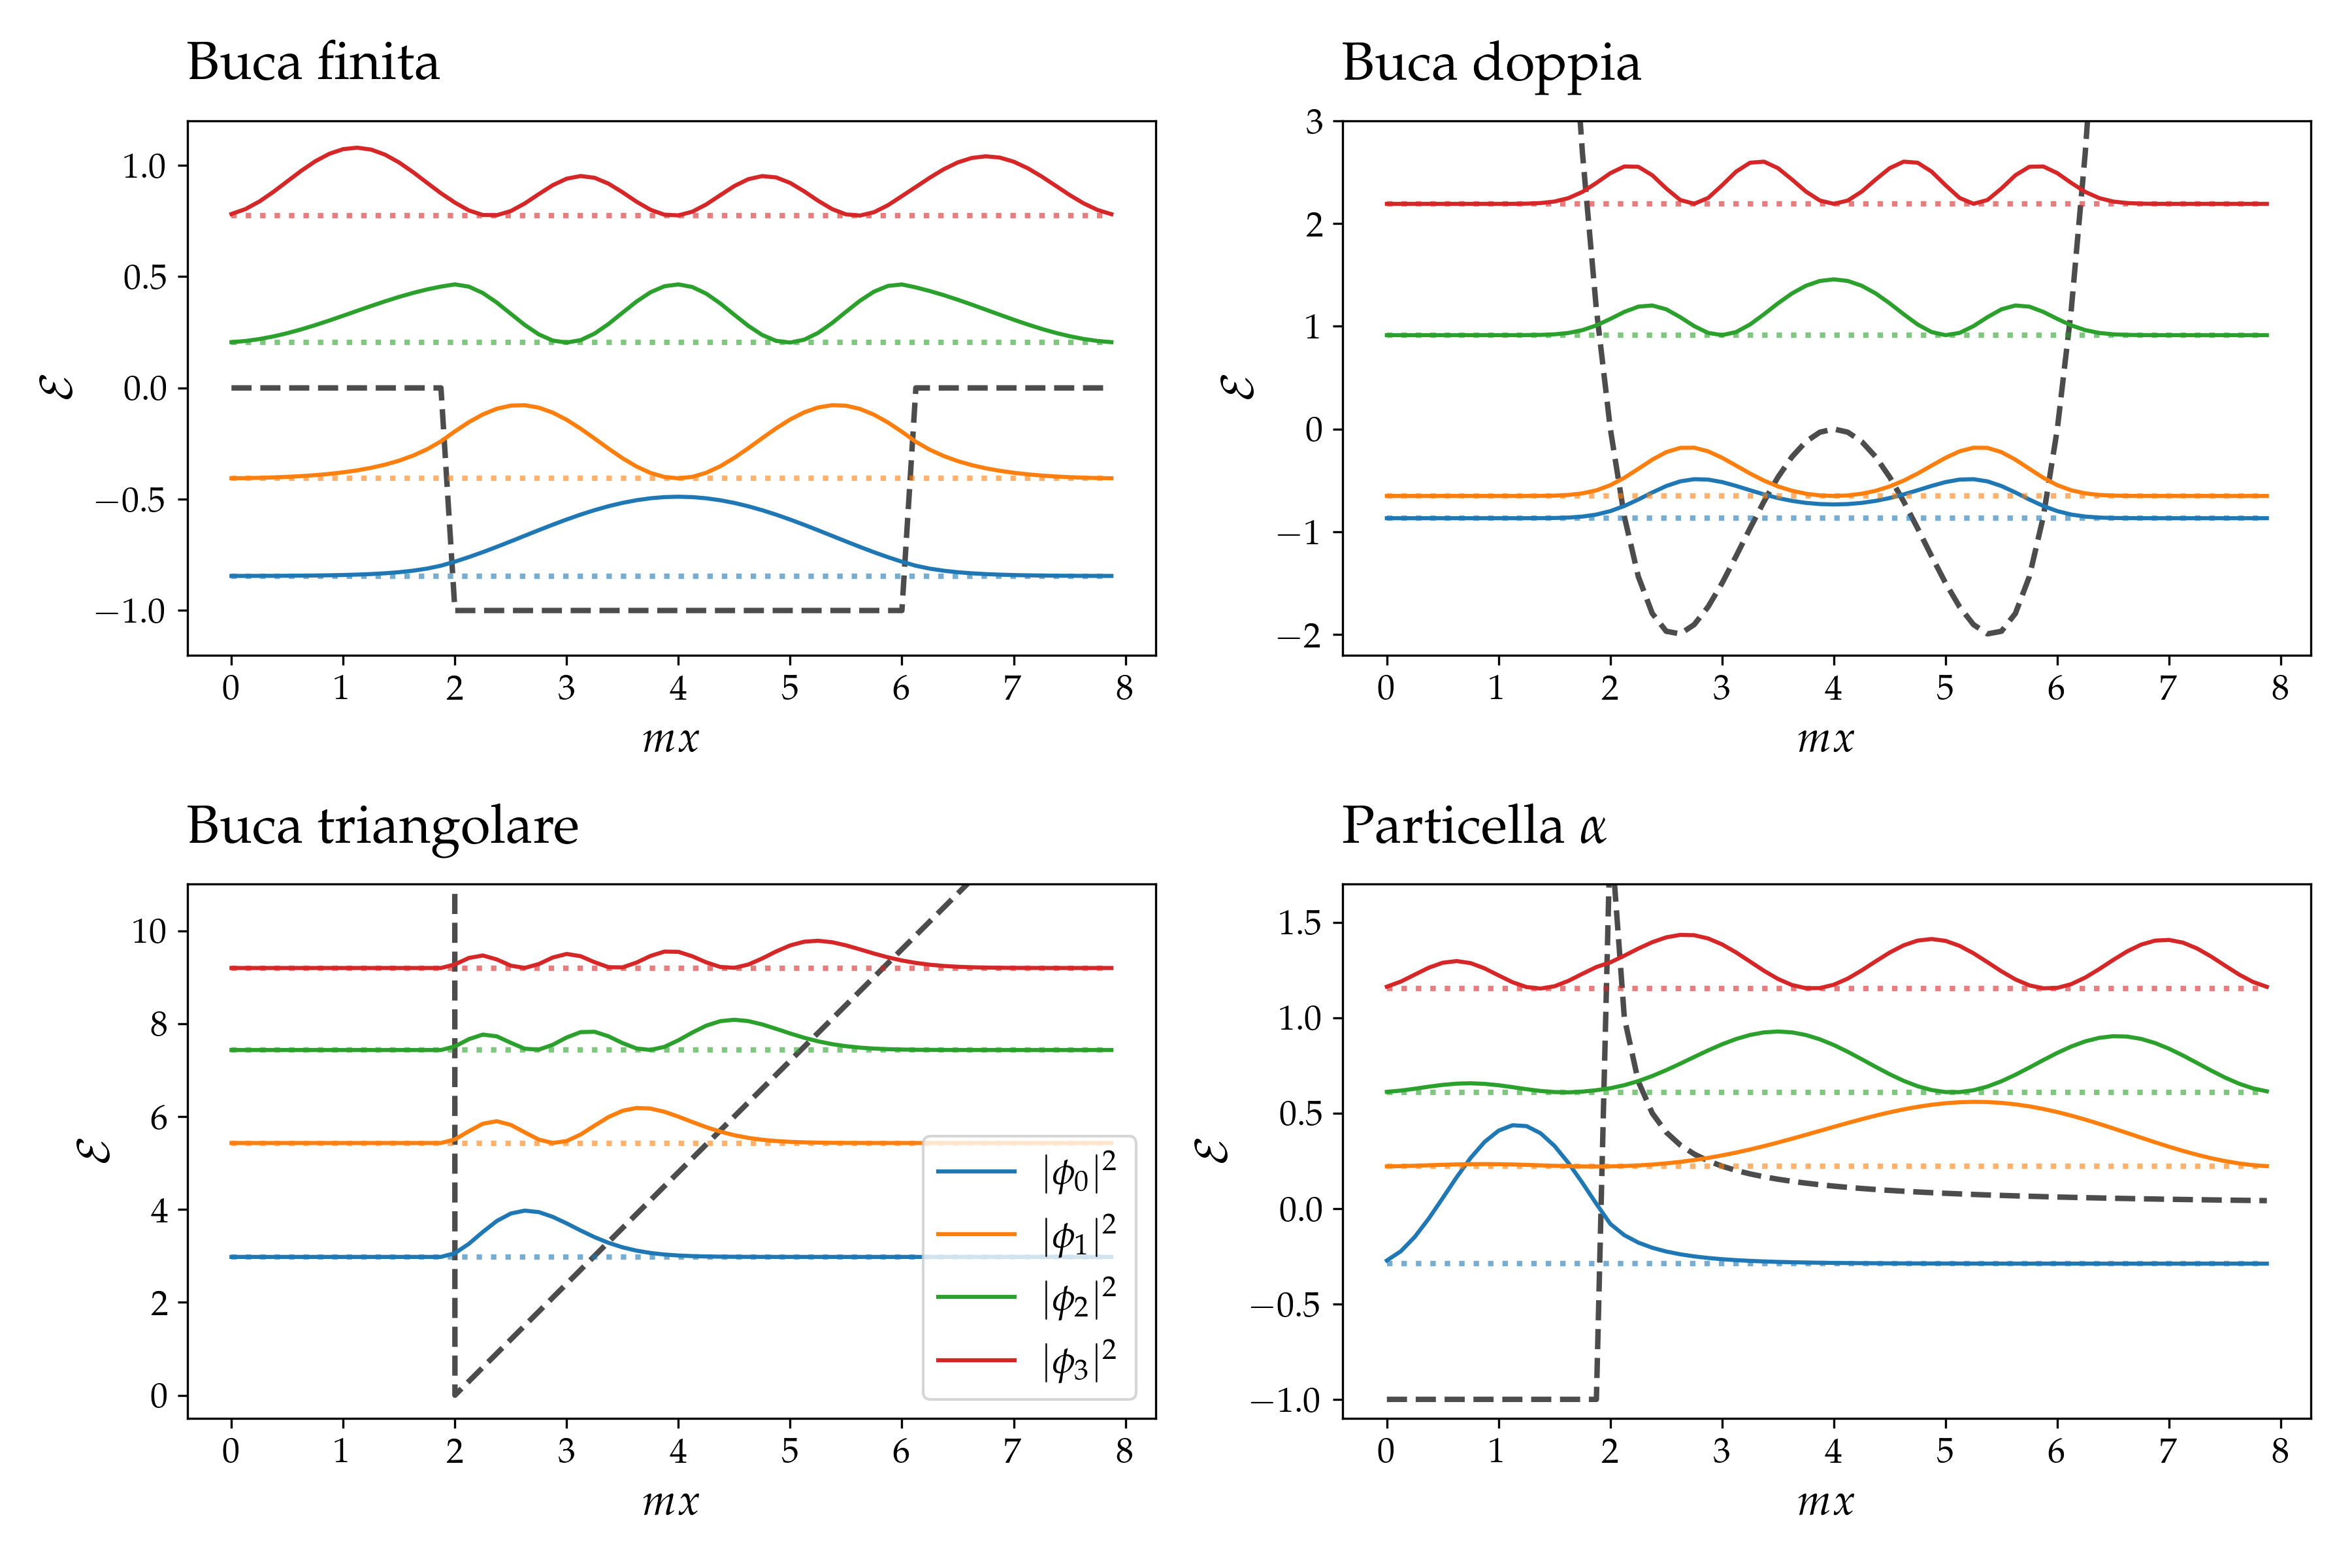
\includegraphics[width=\linewidth]{images/18/comp_Vs.png}
    \caption{Per differenti potenziali statici mostriamo il modulo quadro dei primi quattro autostati.\\
    Si osservi la quasi degenerazione nel grafico relativo alla \textit{double well}, simile a quella descritta nella sezione precedente: il sistema è ancora una volta una buca doppia, con una barriera di potenziale che la divide. Si presentano quindi gli stati quasi degeneri.}
    \label{fig: Diff Pot}
\end{figure}

\newpage














\section{Esercizio 7.2.1}



\subsection{Problem Statement}
Scrivi un programma che implementi lo schema RK4 per risolvere l'equazione di Schrödinger per un pacchetto d'onda incidente, situato in posizione $y$ al tempo iniziale $0$, con momento $p$:$$\psi(x,0) = \mathcal{N} \exp\left(-\frac{|x-y|^2}{\sigma^2}\right) e^{ip \cdot x}$$Normalizza il pacchetto d'onda all'unità.  Per semplicità, definisci un reticolo regolare con la stessa spaziatura per le direzioni $x$ e $y$, con $L_0 = L_1 = L$, $a_0 = a_1 = a$ e $N_0 = N_1 = N = 64$ (mentre sviluppi il codice usa un $N$ ancora più piccolo).  Utilizza i seguenti parametri fisici:
\begin{center}
    $mL = 8$, $y = (L/4, L/2)$, $\sigma m = 0.5$, $p = (p_0, 0)$, $p_0 L = (2\pi)6$.  
\end{center}

\noindent Risolvi l'equazione di Schrödinger fino a $\tau \simeq 0.6$ per i seguenti casi:  
\begin{itemize}
    \item \textbf{Pacchetto d'onda libero}: $V(x,t) = 0 \quad \forall x,t$.  
    
    \item \textbf{Effetto tunnel}: crea una parete lungo l'asse $y$ (perpendicolare alla direzione del moto) con spessore $a$ (o $2a$) situata al centro del reticolo, $L/2$, di ampiezza $32m$, ovvero:
    $$V(x,t) = \begin{cases} 32m & x_0 = [L/2, L/2+a], \forall x_1, t \\ 0 & \text{altrove} \end{cases}$$
    
    \item \textbf{Singola fenditura}: pratica un foro, centrato a $(L/2)$ e di dimensione $4a$, nella parete precedente.  
\end{itemize}
Studia l'evoluzione temporale tracciando $|\psi(x_0, x_1, t)|^2$ usando \textit{contour plots} a, per esempio, $mt = 0.0, 0.2, 0.4, 0.6$. Prova a realizzare anche un'animazione.\\
Per l'effetto tunnel considera di tracciare la norma della funzione d'onda lungo la direzione del moto (asse $x$), mentre per l'esperimento della singola fenditura tracciala a destra della fenditura, come se fosse uno schermo o un rivelatore.  

\subsection{Premessa Teorica}
Il problema si presenta come del tutto simile a quello precedente, però in particolare desideriamo andare a studiare l'evoluzione temporale del sistema, con la possibilità anche di introdurre potenziali non statici (dipendenti dal tempo).
Inoltre passiamo all'indagine di sistema bidimensionali, in cui possiamo effettivamente testare alcune configurazioni di reale approssimazione ad alcuni fenomeni fisici. 


\subsection{Metodi Numerici e Algoritmi}
Ci sono alcune caratteristiche che rendono questo esercizio diverso da quello del Cap. \ref{Cap. Schr t-indep}:
\begin{itemize}
    \item Si tratta di una discretizzazione su un reticolo 2D, quindi ci saranno due termini $a_i$ che determineranno questa risoluzione. Decidiamo di settare entrambi uguali.
    \item È necessaria la linearizzazione della funzione d'onda per la valutazione del laplaciano discretizzato: lavorando con una matrice di grande dimensioni l'operazione più dispendiosa diventa quella di conoscere il valore della fdo nei siti vicini. Con la programmazione in linguaggio \textit{python} è utilissimo l'aiuto della libreria \textit{numpy} che incorpora un metodo che ci permette proprio di traslare il vettore di una posizione (incorporando intrinsecamente le condizioni al contorno periodiche), consentendo la valutazione necessaria in forma vettoriale e ottimizzata computazionalmente.
    \item Se con l'equazione in forma \textit{t-independent} siamo riusciti a riscrivere il problema come una ricerca degli autovalori, in questo caso sarà necessario risolvere esplicitamente l'equazione differenziale ricorrendo ai metodi già studiati nei capitoli precedenti: il metodo più robusto è risultato essere quello di RK4, lo scegliamo quindi per la soluzione.\\
    Dopo aver portato in forma adimensionale tutta l'equazione, la soluzione, con l'ausilio di RK4, diventa:
    \begin{equation*}
    \psi(\vec x, t+\Delta \tau) = \psi(\vec x,t ) + \frac{\Delta \tau}{6} (\psi_1 + 2 \psi_2 +2 \psi_3 + \psi_4)(\vec x) + O(\Delta \tau^5)
    \end{equation*}
    \begin{align*}
        \psi_1(\vec x) & = -i H_m \psi(\vec x) \\
        \psi_2(\vec x) & = -i H_m \big[\psi(\vec x) + \psi_1(\vec x) \Delta \tau/2 \big] \\
        \psi_3(\vec x) & = -i H_m \big[\psi(\vec x) + \psi_2(\vec x) \Delta \tau/2 \big] \\
        \psi_4(\vec x) & = -i H_m \big[\psi(\vec x) + \psi_3(\vec x) \Delta \tau \big]
    \end{align*}
    
    che definisce l'i-esimo step temporale.\\
    Sarà utile assicurarsi che il nostro algoritmo RK4 sia in grado di lavorare con matrici, facendo evolvere tutti i punti contemporaneamente, poiché questa implementazione si traduce in un enorme e indispensabile vantaggio computazionale. 
\end{itemize}


\subsection{Risultati e Discussione}
In generale ho deciso di aumentare la definizione della griglia a $128\times128$, quindi anche alcuni altri parametri sono stati modificati per adeguarsi o per preferenze grafiche: nonostante queste scelte tutti gli esercizi sono stati svolti rigorosamente e presentano dei risultati coerenti e che mi propongo di mostrare qui di seguito.

\medskip\noindent
I parametri modificati sono:
\begin{align*}
    p_0L = (2\pi)20 , \tau =0.4
\end{align*}

\noindent I plot (statici) che si mostreranno di seguito sono fermoimmagini delle relative animazioni. Sono stati catturati come rappresentazioni della $\psi(x, y, t_i),\ t_i\in [0, \tau]$ combinati con il potenziale $V(x, y, t_i)$ (con una trasparenza del $50\%$). Queste figure danno una chiara immagine del fenomeno, ma hanno il difetto di essere disegnate senza mantenere la normalizzazione della \textit{colormap}: ogni plot ha rinormalizzato la scala di colori della \textit{heatmap} usando il valore massimo presente nella matrice in quell'istante, non è quindi possibile confrontare come si diffonda la distribuzione di probabilità totale (chiaramente normalizzata a 1 in ogni momento), poiché due colori uguali su plot diversi non rappresentano lo stesso valore della $\psi$. Per un potenziale statico invece questo tipo di discorso non vale, e chiaramente esso rimane uguale a sé stesso in ogni istante.

\medskip\noindent
Vi sono alcuni dettagli in più che riguardano le animazioni e i plot statici, ma ne discutiamo nell'Appendice \ref{App: rappr schr}: queste note sono importanti per chiarire alcune scelte nelle rappresentazioni e le principali differenze che sussistono tra le immagini che seguono e le animazioni riportate nella repo Github. Ritengo che questo discorso possa limitarsi ad un approfondimento e che si possa rilegare all'interesse del lettore, nonostante io reputi queste animazioni la parte più interessante e completa prodotta nell'intero corso. Anche per questa motivazione si conserva una discussione più chiara ad una sezione separata come quella in appendice.


\subsubsection{Particella libera $V(x)=0, \forall \boldsymbol x, t$}
La particella evolve sul reticolo come particella libera: mantiene la forma di gaussiana simmetrica lungo ciascun asse indipendentemente, ma non è più simmetrica nel piano, poiché la campana si allarga in maniera differente lungo le due direzioni (la sua curtosi diventa $k<3$).\\
Il principio di indeterminazione agisce in maniera chiarissima in questo caso, la precisione che avevamo nell'istante iniziale sulla posizione della particella sta diminuendo al passare dei secondi poiché essa si comporta come un'onda che si propaga nello spazio!

\begin{figure}[H]
    \centering
    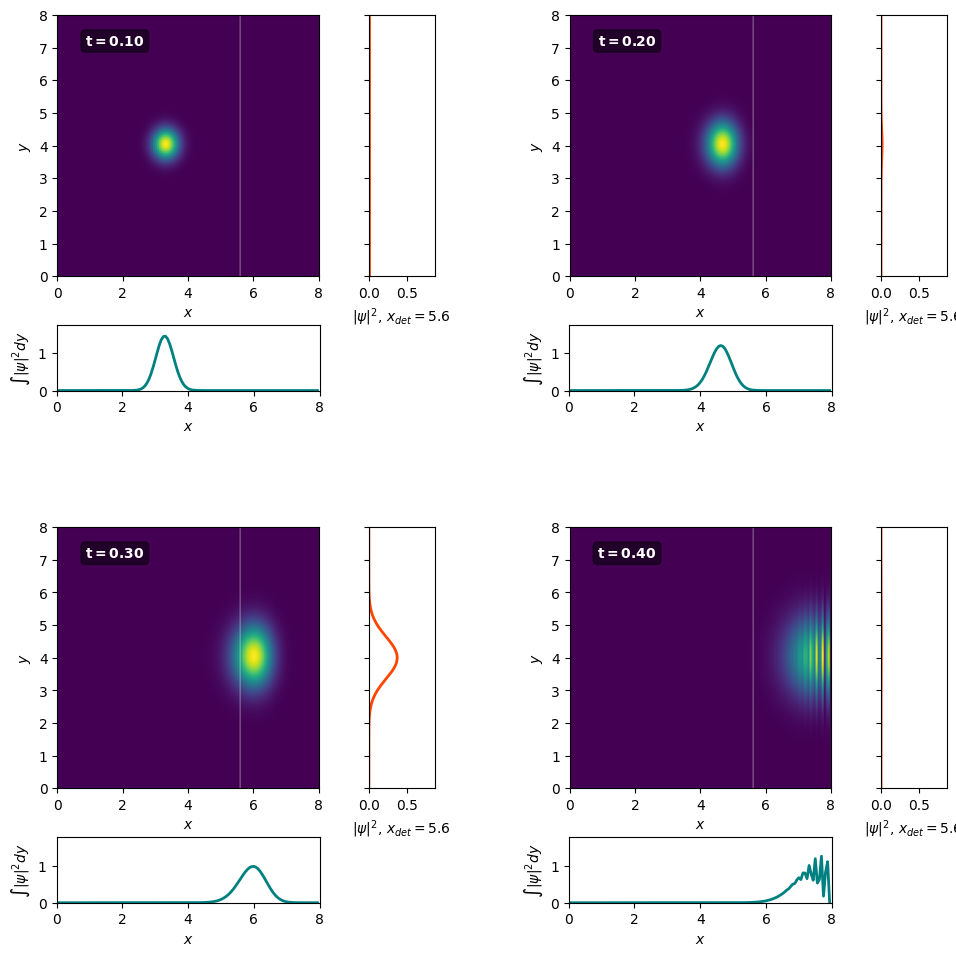
\includegraphics[width=0.8\linewidth]{images/19/pot/free_part_pot.png}
    \caption{Particella libera.}
    \label{fig: part_libera}
\end{figure}

\subsubsection{Effetto tunnel}
Per questo esempio prendiamo in considerazione una barriera di potenziale posizionata nel centro del dominio:
\begin{align*}
    V(x) = \begin{cases}
        V_0 \quad &x_{pos}\le x \le x_{pos} + d\\
        0 \quad &\text{altrimenti}
    \end{cases}    \quad \qquad\forall\ \boldsymbol y, t
\end{align*}

\noindent dove $x_{pos}$ è la posizione sull'asse x di questa barriera, mentre $d$ la profondità che abbiamo settato.\\
Ho impostato il livello $V_0$ del potenziale in maniera tale che ci fosse un buon equilibrio tra ciò che viene riflesso e quello che invece attraversa (tunneling); se il momento iniziale non è sufficiente, la particella verrà sempre più respinta dalla barriera, fino al punto che per lei sarà impossibile attraversarla perché nello spessore in cui abbiamo la regione proibita, dove $V(x)>E$, la funzione d'onda diventa evanescente e decade esponenzialmente, in maniera tale da confinare definitivamente la fdo nella regione a sinistra.  

\medskip\noindent
Il fenomeno è ben visibile in Fig. \ref{fig: bar_fin}.


\begin{figure}[H]
    \centering
    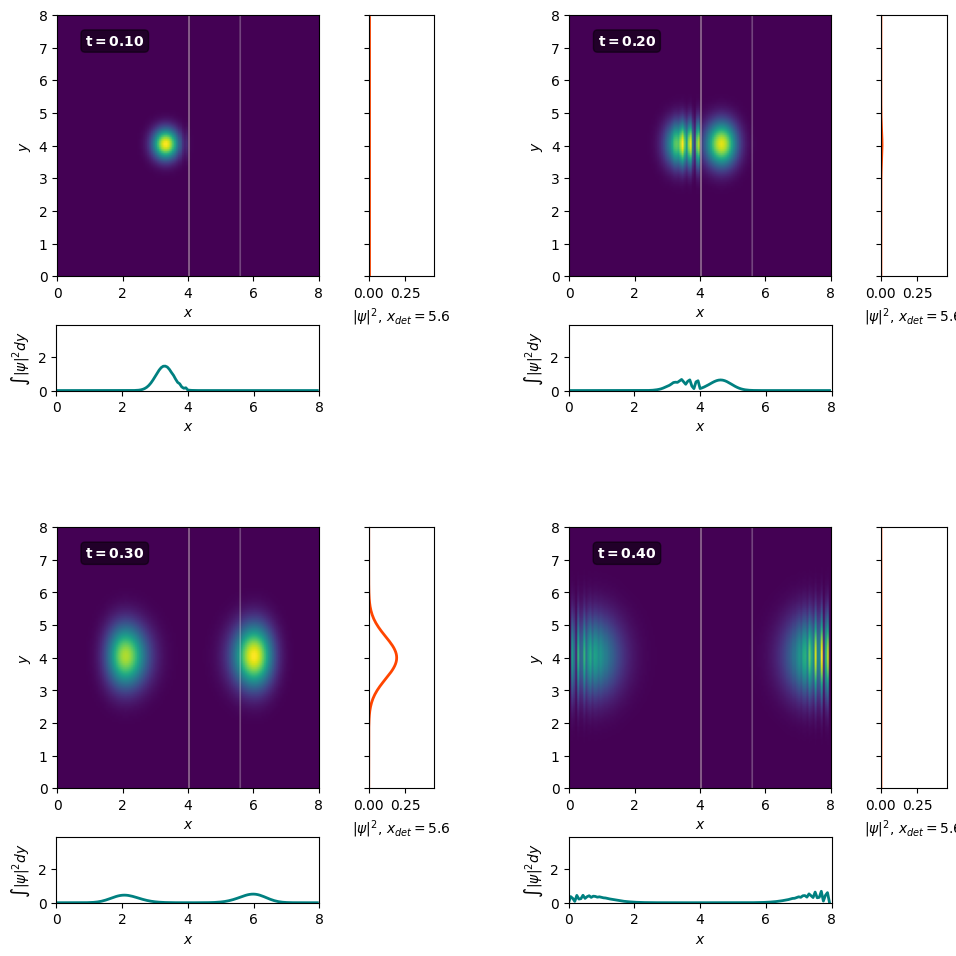
\includegraphics[width=0.8\linewidth]{images/19/pot/finite_wall_pot.png}
    \caption{Barriera finita e effetto tunnel.}
    \label{fig: bar_fin}
\end{figure}


\subsubsection{Singola (e doppia) fenditura}
Gli esperimenti con le fenditure sono il biglietto da visita per la QM, spesso il primo approccio con essa. In essi si può osservare direttamente e inequivocabilmente la natura ondulatoria della materia e si dà spiegazione di alcuni esperimenti particolarmente eclatanti.

\medskip\noindent
Quando un pacchetto d'onda interagisce con una barriera di potenziale infinita, osserviamo una riflessione totale dello stesso; se immaginiamo di forare questa barriera, permettendo quindi alla fdo di passare, si osserva il fenomeno di diffrazione, tipico di tutti i fenomeni ondulatori, e i relativi pattern di interferenza. Il plot che ho posizionato sulla destra, discusso in appendice, è un sensore, che risulta molto utile per simulare un esperimento di laboratorio e i possibili risultati che ci aspetteremmo di ritrovare su uno schermo.\\
In Fig. \ref{fig: one_slit} e \ref{fig: doub_slit} si osserva ciò che abbiamo discusso. La differenza fra i due fenomeni sta nel fatto che se nella singola fenditura ci si limita ad osservare la diffrazione, spiegata con il principio che ha una spiegazione nel principio di Huygens-Fresnel, cioè un fenomeno di autointerferenza, nella doppia fenditura questo si sovrappone all'interferenza che due sorgenti di diffrazione operano l'una sull'altra. Quello che si rileva è che per entrambi si generano figure di costruttive e distruttive, visibili come bande scure o chiare al di là della barriera. Si noti che la barriera di potenziale è impostata in maniera tale da essere sufficientemente energetica per essere considerata infinita; impostando valori ancora maggiori si osserva che il programma, nella sua operazione di risoluzione della PDE, si rompe, causando errori numerici e non conservando più la norma della fdo.

\begin{figure}[H]
    \centering
    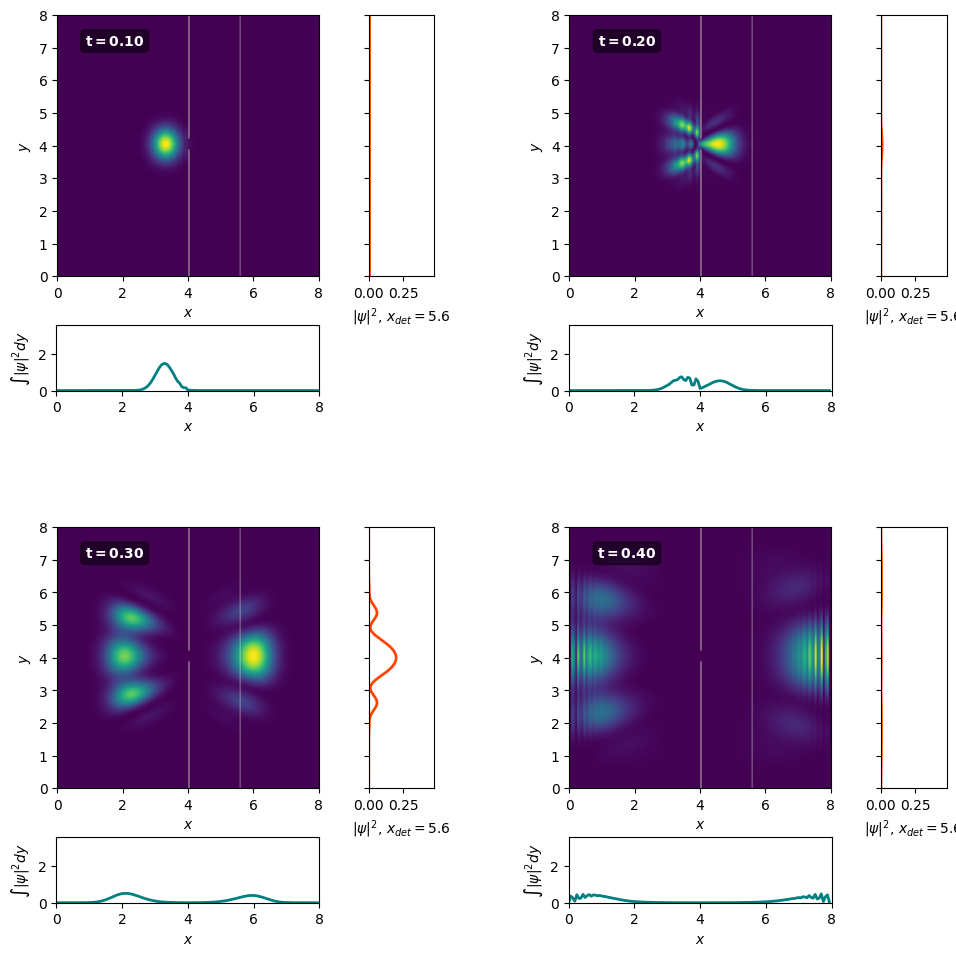
\includegraphics[width=0.65\linewidth]{images/19/pot/one_slit_pot.png}
    \caption{Esperimento a fenditura singola.}
    \label{fig: one_slit}
\end{figure}

\begin{figure}[H]
    \centering
    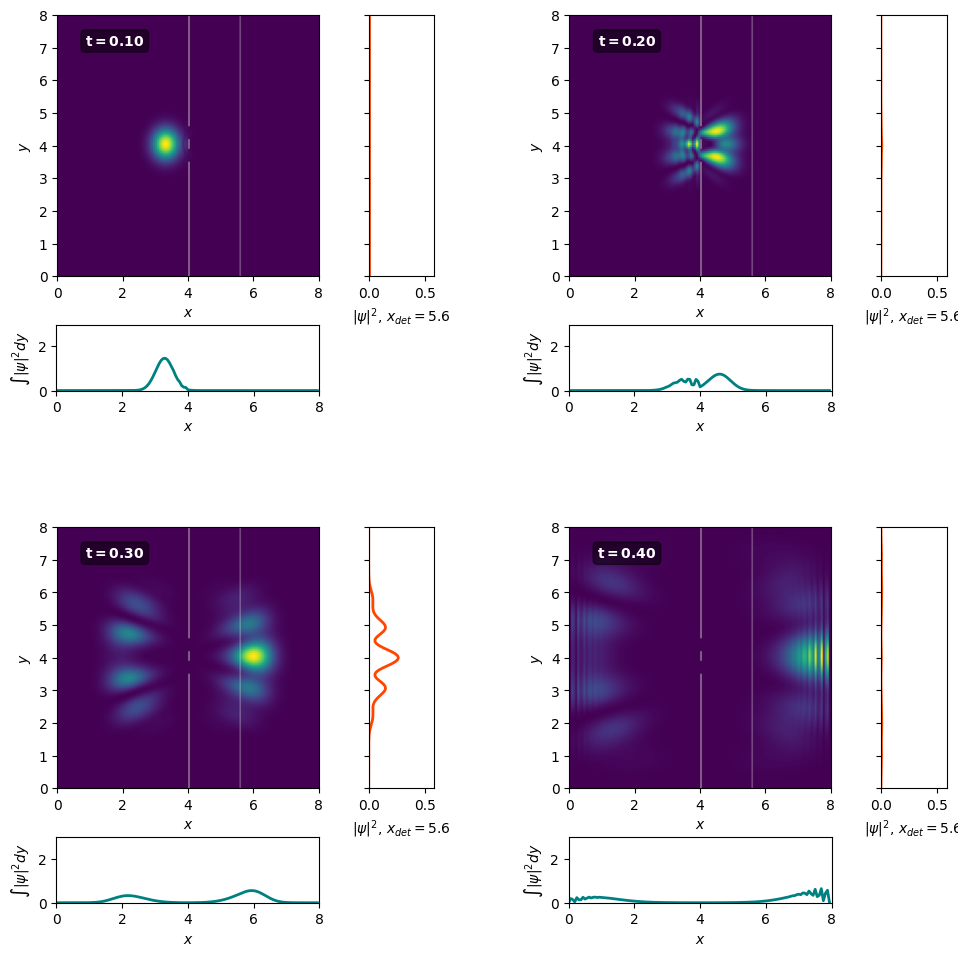
\includegraphics[width=0.65\linewidth]{images/19/pot/double_slit_pot.png}
    \caption{Esperimento della doppia fenditura.}
    \label{fig: doub_slit}
\end{figure}

\noindent Nello studio del fenomeno ho voluto sperimentare anche con altri casi che generalizzano i due precedenti: il reticolo di diffrazione e il singolo ostacolo.

Per quanto riguarda il reticolo di diffrazione esso è il caso n-esimo di diffrazione, con infinite, idealmente, sorgenti di onde sferiche, che sono le $n$ fenditure che si alternano costituendo il reticolo. Ciò che si rileva è la presenza delle fasce di interferenza, equivalenti a quelle delle esperienze già discusse.

L'ostacolo rappresenta un caso complementare alla singola fenditura: per il \textit{Principio di Babinet} essi provocano un fenomeno identico, andando a far interagire per interferenza l'onda incidente, in maniera però differente. Questo è il fenomeno osservabile con un ostacolo lineare sottile (un laser con un capello) oppure con un piccolo bersaglio circolare (si osservano i famosi \textit{Dischi di Airy}). 

\bigskip

\begin{figure}[H]
    \centering
    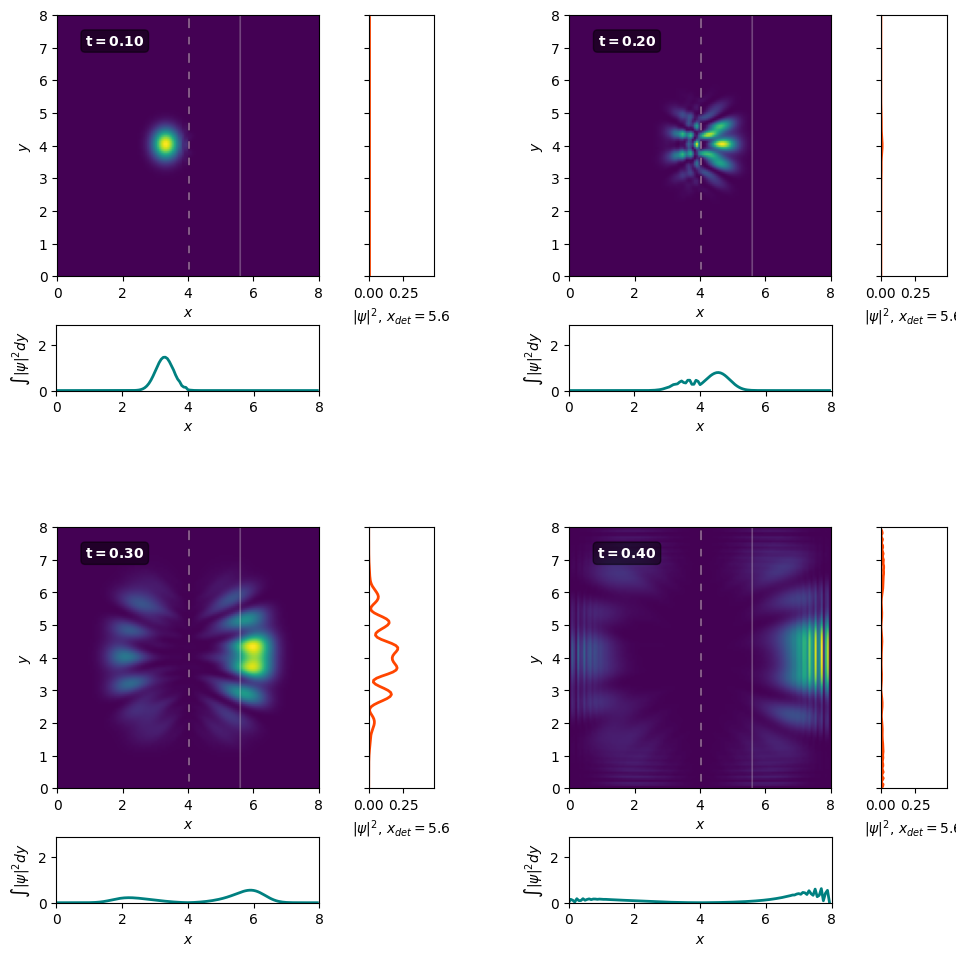
\includegraphics[width=0.7\linewidth]{images/19/pot/diff_grate_pot.png}
    \caption{Reticolo di diffrazione uniforme, ortogonale alla direzione di propagazione.}
    \label{fig: diff_grate}
\end{figure}


\begin{figure}[H]
    \centering
    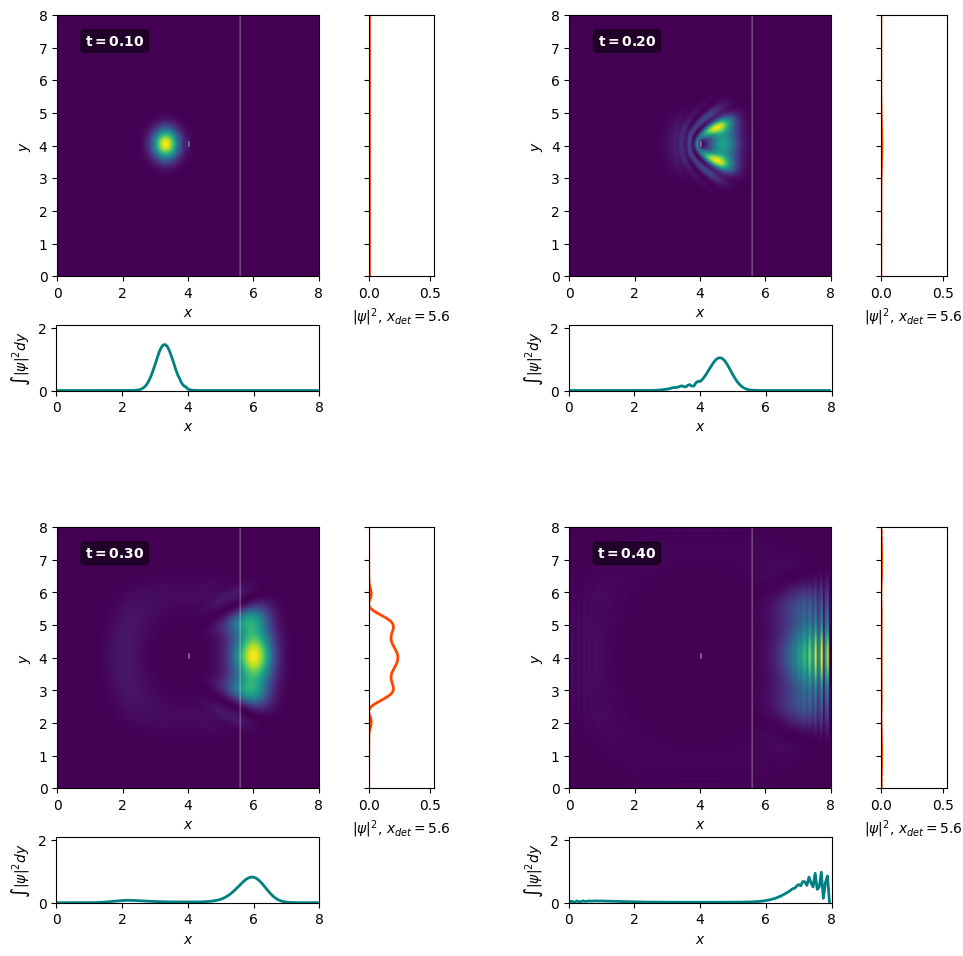
\includegraphics[width=0.7\linewidth]{images/19/pot/one_obst_pot.png}
    \caption{Diffrazione con un ostacolo.}
    \label{fig: diff_grate}
\end{figure}


\subsubsection{Casi di studio su potenziali alternativi}
Propongo in questa ultima sezione conclusiva alcuni casi di rilevanza fisica e che comunque presentano delle particolarità interessanti.

\bigskip

\noindent \textbf{Potenziale della particella alfa (\textit{Potenziale di Gamow}):}\\
\noindent Lo abbiamo già discusso nell'esercizio precedente; rimandiamo a quella sezione l'approfondimento generale. Proponiamo qui le soluzioni per un potenziale alfa configurato in due modi differenti: la barriera del potenziale coulombiano è più o meno intensa, risultando nella possibilità o meno di effetto tunnel e quindi esistenza di autostati esterni al nucleo (la particella alfa viene emessa e fugge), mantenendo il momento della particella uguale.\\
Nei grafici di seguito viene omessa la visualizzazione del potenziale, poiché è troppo opaco e non permette una chiara visibilità sul problema.

\begin{figure}[H]
    \centering
    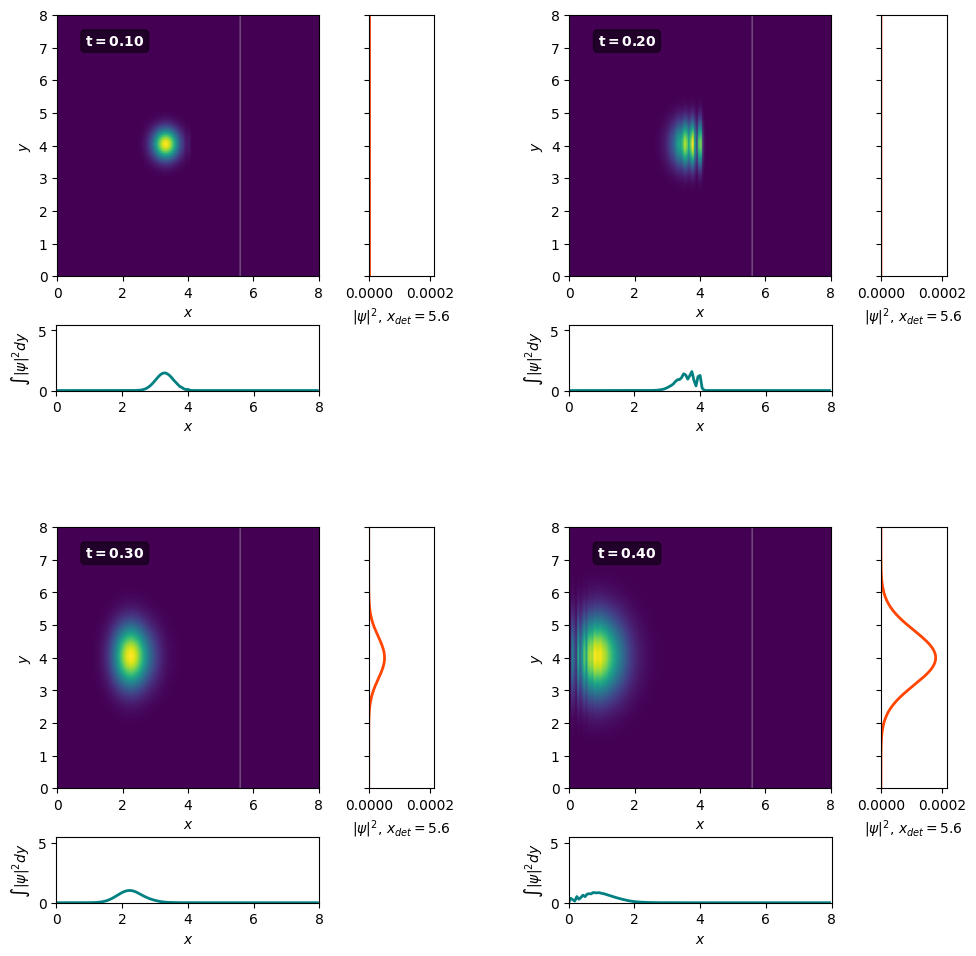
\includegraphics[width=0.65\linewidth]{images/19/no_pot/alpha_p_V0.png}
    \caption{Particella alfa confinata nella buca di potenziale (nucleo).}
    \label{fig:placeholder}
\end{figure}

\begin{figure}[H]
    \centering
    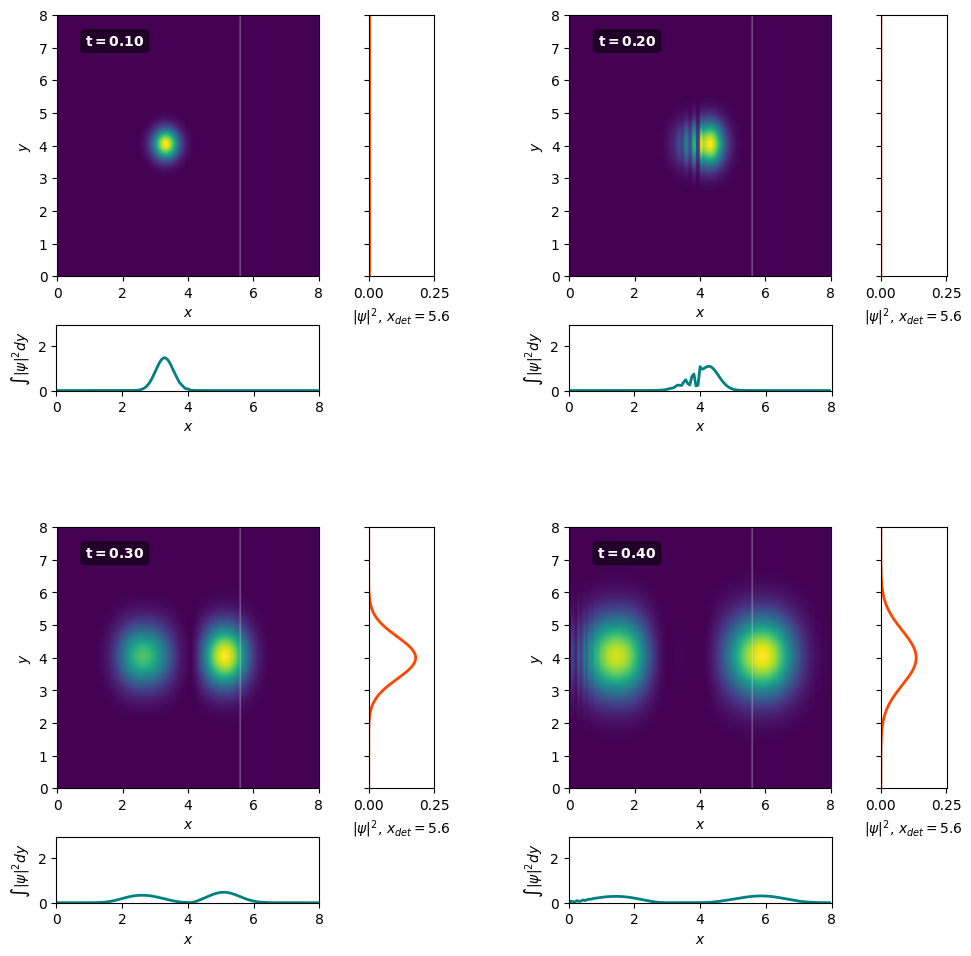
\includegraphics[width=0.65\linewidth]{images/19/no_pot/alpha_p_hV0.png}
    \caption{Particella alfa che riesce a fare tunneling e viene emessa dal nucleo.}
    \label{fig:placeholder}
\end{figure}


\noindent \textbf{Proiettile:}\\
\noindent Ho desiderato sperimentare anche con un potenziale variabile nel tempo introducendo un proiettile energetico che si muove nella stessa direzione e senso opposto rispetto al nostro pacchetto d'onda: si ottiene un urto frontale che distrugge l'integrità della campana gaussiana provocando, ancora una volta, dei pattern di interferenza. 

Questo non è un vero è proprio caso di potenziale \textit{t-dependent}, poiché a variare non è il valore $V_0$, bensì la localizzazione nel dominio, dell'ostacolo. Suppongo questo caso possa essere descritto come un esempio particolare di collisione con un ostacolo fermo di dimensioni analoghe, ma aumentando il momento $p_0$ della particella per combaciare con quello del moto relativo dei due.\\
Di seguito i risultati dell'analisi.

\bigskip

\begin{figure}[H]
    \centering
    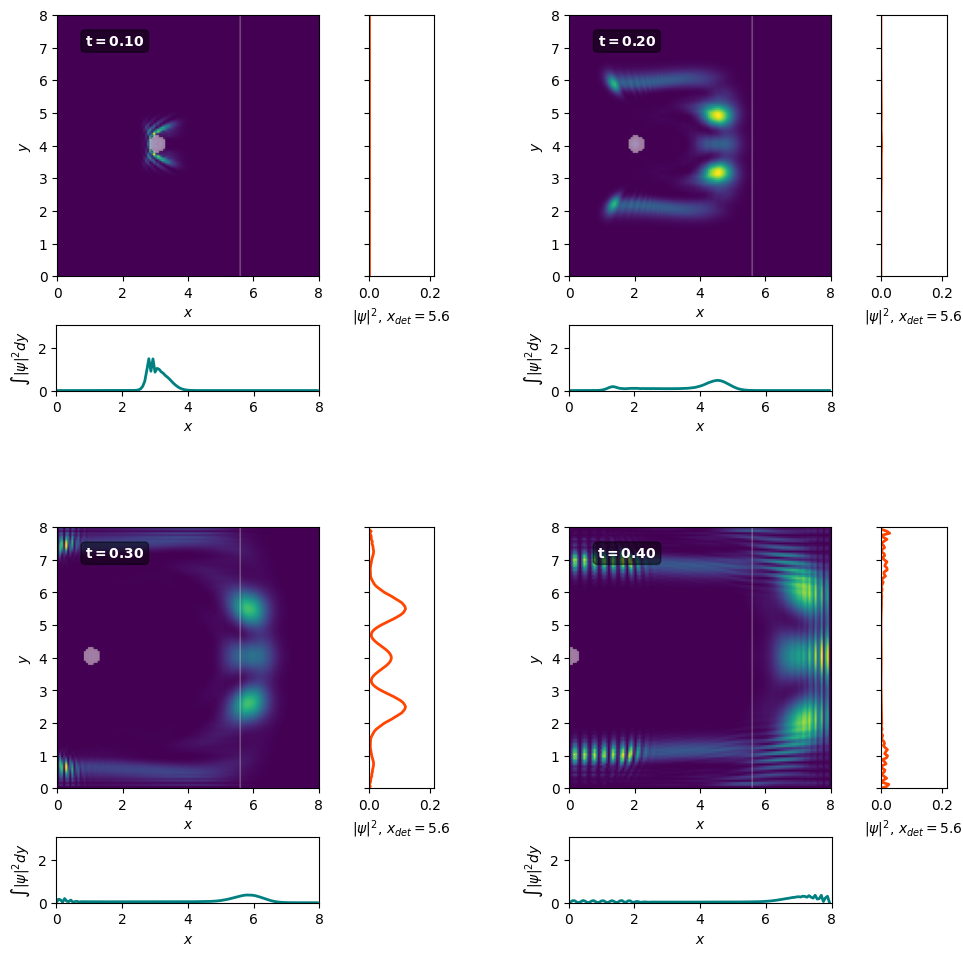
\includegraphics[width=0.8\linewidth]{images/19/pot/bullet_pot.png}
    \caption{Proiettile sferico di potenziale.}
    \label{fig: bullet}
\end{figure}



\newpage




